\documentclass{article}
\usepackage[utf8]{inputenc}
\usepackage[english]{babel}
\usepackage{amsmath}
\usepackage{amssymb}
\usepackage{setspace}
\usepackage{natbib}
\usepackage{graphicx}
\usepackage{subfig}
\usepackage{comment}
\usepackage[backgroundcolor=pink,linecolor=red]{todonotes}
 \usepackage{fullpage}
\usepackage[hidelinks]{hyperref}
\usepackage{xcolor}


%\singlespacing
\onehalfspacing
%\doublespacing
%\setstretch{1.1}

\newcommand{\plr}[1]{\todo[linecolor=blue,backgroundcolor=blue!25,bordercolor=blue]{#1}}
\newcommand{\jgg}[1]{\todo[linecolor=green,backgroundcolor=green!25,bordercolor=black]{#1}}

\begin{document}

\linespread{1.5}

JARGON WE SHOULD THINK ON ??

Trait | Phenotype = Probably Trait

effect loci | QTL | causal: = ??
 
Original Lakes | $P_{1}$, $P_{3}$, $P_{3}$ = ?

Migration Rate | Introgression = ?

\section{Abstract}

\todo{Do last.}

\section{Introduction}

\todo{Take out any "we's" and be more specific}

% Jared's general notes for formatting

%\plr{``citep'' for ``cite in parentheses''. (and, citations come before the punctuation)}
%\plr{in latex, use ` `words' ' to get the open- and closed-double quotes (not the double-quote character)}
%\plr{"citet" for "cite, as part of the text"}

\jgg{Starting a paper is awkward, help}
The rate and tempo of evolution remains largely unknown.
Today, we have found multiple examples as evidence of rapid evolution 
in tens of generations or fewer.
Biologists are now starting to address the complexity behind ecological speciation. 
\jgg{Peter and Bill: Could use help with examples of rapid evolution and the story leading up to stickleback right here}

Recently, multiple instances of similar (parallel) underlying genetic basis of rapid local adaptation has brought about 
questions surrounding the origins of adaptive alleles.
A empirical model is the alaskan populations of freshwater and marine Ninespine Stickleback fish.
In 1964, The Great Alaskan Earthquake caused an uplift of Middleton island and in turn,
introduced a group of freshwater ponds around the perimeter of the island. 
Quickly inhabited by the surrounding marine population of Stickleback,
\citet{LescakE7204} observed significant phenotypic changes in less than 50 years that appear to be 
parallel to freshwater stickleback that have been separated for over $13,000$ years.
In freshwater stickleback, the number of lateral plates are reduced
and the opercle shapes shows the same expansion of the dorsal region and reduction of the ventral region.
\jgg{Bill - more specifics about Bill, Suzie, Kristin  \& or Thom's papers .. ? }
These results leave us with questions surrounding the nature of rapid adaptation.
Does convergent evolution breed it's own solution (haplotype) for every new selective pressure, 
or can these solutions can be efficiently shared across multiple sub - populations facing similar selective pressures. 

The leading hypothesis for stickleback is that rather than acting on new mutations, 
adaptation to freshwater environments is sped up through selection on standing genetic variation (SGV) found in marine populations. 
\jgg{Bill: maybe you could make this section a little more specific}
One clear example of this is the gene \textit{eda} 
which has been shown to regulate the number of lateral plates. 
While this gene arose millions of years ago, it is found in freshwater ponds which have formed much more recently.
Novel evidence from natural populations has provided evidence that most regions of the genome that distinguish marine-freshwater genetic differences share this pattern. \cite{Nelson2017} 
\citet{schluter2009genetics} 
suggested the ``transporter''-hypothesis.  
This outlined the flow of freshwater alleles into marine populations through offspring of hybridization events.
It suggests freshwater haplotypes are distributed though marine individuals and are continually selected upon in introduced freshwater populations.
The continued selection on freshwater favored alleles and introgression between the two sub-species,
allows the marine to maintain the freshwater haplotype dispersed in low frequency among its' individuals. 
Once a new freshwater environment is introduced and inhabited by marine individuals who carry freshwater adapted alleles, selection reconstructs the freshwater haplotype. \cite{schluter2009genetics} 
An alternative to this hypothesis is that individuals from other freshwater environments migrate directly to the new environments, 
and their haplotype is passed down directly. 
This hypothesis has been shown to be unlikely due to finding a high frequency of freshwater alleles in the ocean,
and almost no freshwater individuals.

\plr{Bring up the possibility of more than one freshwater haplotype here.}
\jgg{Re: should I? Doesn't Thom's work and parallel above suggest they have the same alleles?}

If selection on SGV is key in rapid adaptation, 
many questions are brought to light concerning the surrounding population genetics parameters and underlying genomic architecture.
How rapidly can selection act on standing genetic variants at a given value of migration, $M$?
How many alleles underly a certain trait? (expand here)
Furthermore, how can we infer causal loci for regions of the genome that must be driving the rapid adaptation, from real data.
Many biologist today make use of genome wide association studies (GWAS) and 
$F_{st}$ across the genome to estimate regions responsible for certain traits. 
Unfortunately, the data can be heavily influenced by the level of introgression and population structure of the samples. 
This being the case, what are the biases we can expect to see in real data for certain levels of introgression. 

There are many different parameters that carry a large impact on the questions above.
\citet{Ralph2015} 
explored the dichotomy of selection on new alleles and those brought in by migrants from a similar selective pressure.
This lead to an understanding of the process by which alleles move from an existing 'patch' to an introduced 'patch' with the 
same selective pressure. 
%read though Peter's paper more and connect it to what we're doing here. 

In this paper, we explore time to local adaptation as a function of migration rate through an environment (marine) with opposing selective pressure. 
Next, we compare to real data and explore how $F_{st}$ data can be impacted by introgression, or lack of.
%Explain what we do and what we find that is important

%We use forward moving simulations to model marine and freshwater populations of stickleback.
%We then observe the effect (focusing on migration and recombination, for now) 
%of different parameters on local adaptation of introduced freshwater environments. 

\section{Simulation Model}

Our simulations are forward-moving evolutionary models which
emulate the geography, selective pressure, and genomic architecture 
of coastal marine and freshwater lake populations. 
Here, we describe the specifics of out model.

\subsection*{life cycle}

For this study, we used a flexible evolutionary framework, SLiM \citep{Haller2017}.
The model-type we used was based off of an extended wright-fisher. 
The simulation life cycle of each generation is as follows.
First, generate offspring by:
(1) choosing parents based on cached fitness values and migration rates, 
(2) performing recombination of parental genomes, 
(3) allow for mutation, 
(4) modify each child by a defined callback. 
Next, offspring become individuals before fitness is evaluated for the next generation.
Finally, the generation counter is incremented. 
The population structure in SLiM can be arranged in any number of subpopulations, 
continuous or discrete, connected by any rate of migration. 

\subsection*{Geography}

What we've modeled geographically is a coastal marine population 
connected by migration to multiple, smaller freshwater populations that are located along the coast.
The population structure for the marine is modeled as a one-dimensional, continuous population
ranging from 0.0 to 10.0.
There are two sets of lakes which represent freshwater populations; 
the first which evolves in parallel to the marine, 
and a set introduced later in the simulation as a subset of the marine. 
Each of the $10$ lakes, $i$, is located along the marine at $i - 0.5$, 
and connected by migration only through the marine environment. 
The marine has $2000$ individuals while 
each of the lakes fluctuate around $200$. 

\begin{figure}
	\begin{center}
  		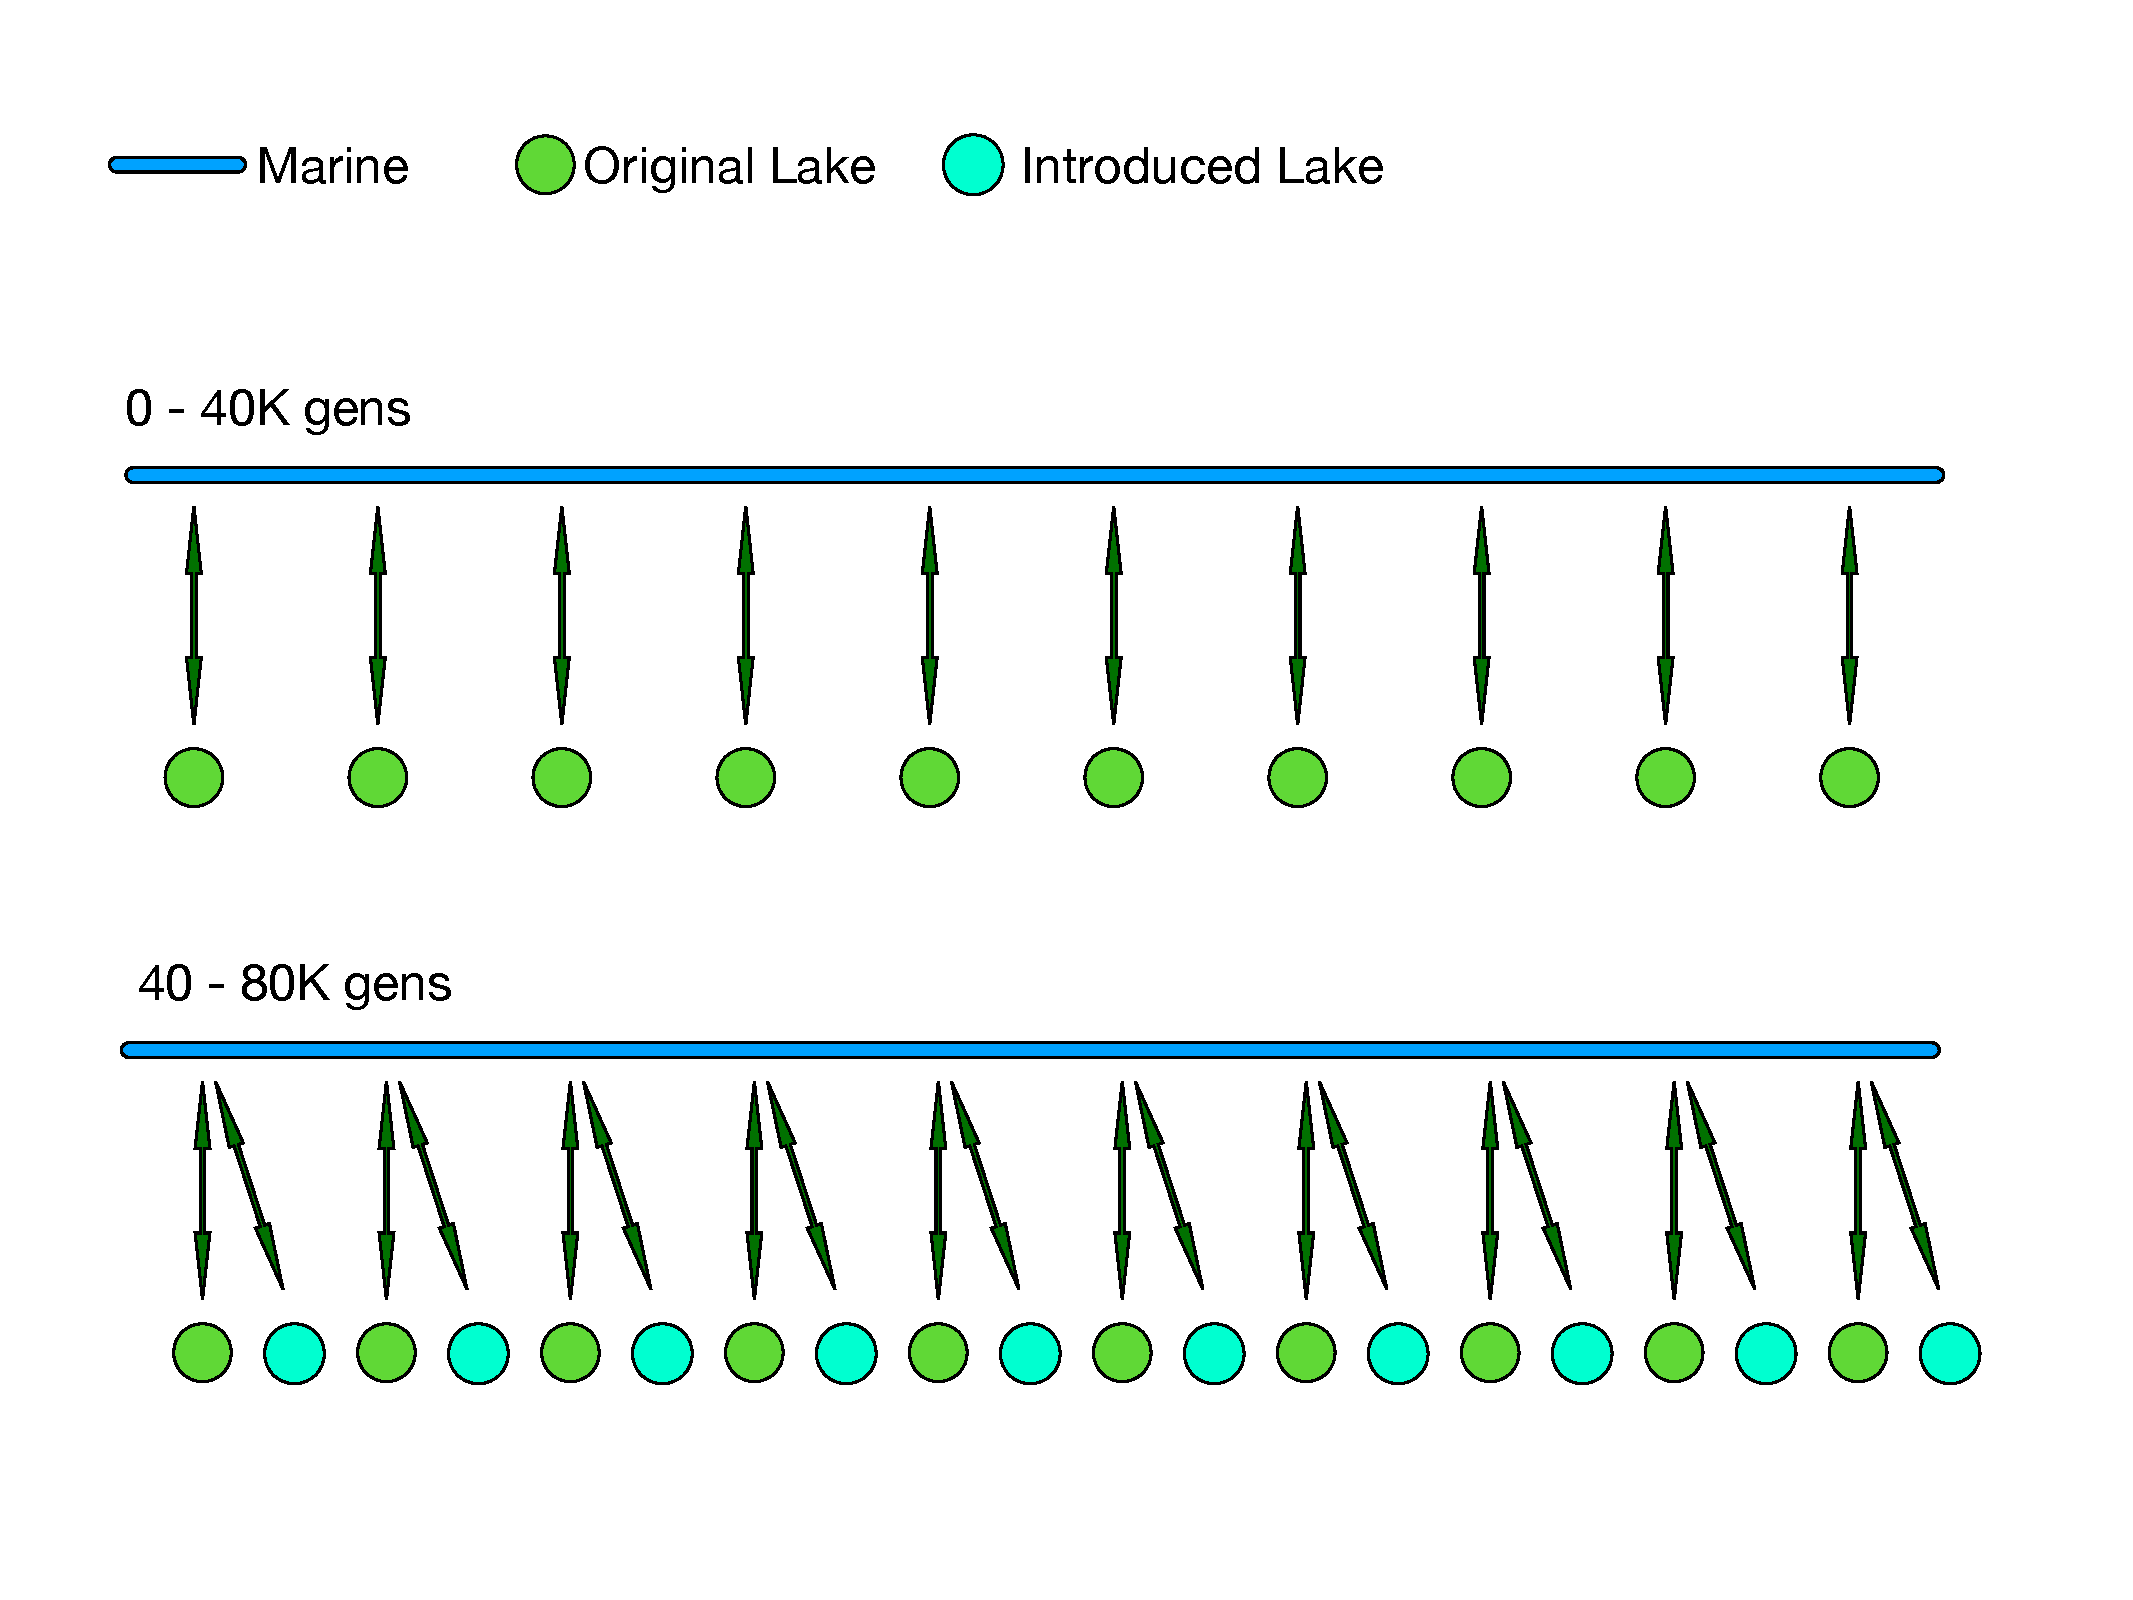
\includegraphics[width=0.6\linewidth]{GeographyDiagram}
  		\caption{A representation of the geographic and evolutionary history of all populations throughout the simulation. 
		The marine is a one-dimensional, continuous population with spatial positions ranging from [0.0 - 10.0]. Each 
		lake$_{i}$ is a discrete population connected by migration only through the marine at position $i - 0.5$. The introduced lakes 
		have the same location and selective pressure as the original lakes, but arise at 40K generations.
		the introduced population is initialized as a copy of all marine individuals to model marine 
		individuals inhabiting a newly created freshwater environment such as the ponds around Middleton Island.
		We then observe the selection process of marine individuals and following generations 
		with the new selective pressure across a range of parameter values. 
		%Migration between the marine and original lakes is 
		%set to $0$ the generation before introduction to avoid direct migrants from original $->$ introduced lakes.
		}
  		\label{fig:Geo}
	\end{center}
\end{figure}

\subsection*{Selective Pressure}

%(TALK ABOUT ADAPTEDNESS and TRADE-OFF), 
% abstracting real fish phenotype with `` trait value "

%Trait value is equal to the sum of the contribution of the effect loci and the loci may be 
%add, dom, recc. Uniformly chosen 

To emulate the freshwater and marine selective pressure, 
we set up a quantitative genetics model in which fitness is phenotypically based. 
Freshwater and Marine environments are distinguished by a single numeric value. 
This number is the optimum trait value for each environment
and acts as a representation of lateral plate number and opercle shape in the stickleback populations.
%The fitness of an individual is then determined by a probability density for a normal distribution 
%at the quantile (?) of the difference between the optimum and the individual's phenotype
We use a Gaussian fitness function, 
where the fitness of an individual with trait $x$ in a population with optimal trait value $x_0$ is:
\begin{align}
    f(x; x_0) &= \exp\left(\frac{(x - x_0)^2 }{ 2 \sigma^2}\right),
\end{align}
with $\sigma = 15$.

Where a trait value, $x$, is also defined by a single numeric value; 
determined as a summation of the selection coefficients of all mutations an individual possesses. 
% no empty lines before equations, usually - they should read like part of the text itself.
%	\[
%{\textnormal{Individual.Phenotype = } \sum_{m \in mutations} \textnormal{m.selectionCoeff}}
%	\]
    
We allow six mutation types which affect phenotype along with one neutral mutation type.
Among the effect mutations; 
there are additive, dominant, and recessive mutations which a ffect phenotype
in either the positive or negative direction. 
The selection coefficients are pulled from a gamma distribution 
with a shape parameter of $1$ and a mean of either $0.5$, or ${-0.5}$. 
\plr{Can just say this in words, no need to have an equation.
    Also, a Gamma with shape 1 and mean 0.5 is an Exponential with mean 0.5.}

%	\[
%\textnormal{Mutation.selectionCoeff = } X \sim \Gamma (1,\pm0.5)
%	\]

\todo{maybe the order of these should be reversed?}
\plr{I agree: first explain how phenotypes are calculated, then say what fitness is.
    Notation suggestion: phenotype for an individual that is heterozygous at loci $H$
    and homozygous derived at loci $D$ is $x = \sum_{\ell \in H} h_\ell s_\ell + \sum_{\ell \in D} s_\ell$,
    where $h_\ell$ is the dominance coefficient for locus $\ell$ (0 for recessive, 1 for dominant, 0.5 for additive),
    and $s_\ell$ is the effect of the derived mutation on the phenotype}

\subsection*{Genomic Architecture}

\plr{This should maybe come before the phenotype.}
In SLiM, the genome is conceptually a linear array of loci defining locations for 
mutations that arise and breakpoints for recombination. 
Genomic elements define a range depicting the types of mutations that can arise, and the ratio at which different mutation types can arise. 
Although still uncertain about how much of the genome is directly associated with the distinguished phenotypes, 
GWAS has indicated clusters of loci (linkage groups? Operon?) along the genome to be causative. 
To mimic this and compare dynamics of neutral vs. effect under selection, 
we create regions of effect. (???)
In these genomic elements of effect, we uniformly allow additive, recessive, and dominant, mutation that can push phenotype in either the positive or negative direction to arise. 
Every genomic position outside of these effect regions only allows for selectively neutral mutations to arise.

In our simulations, there are 10 effect regions of size 100 loci, uniformly placed between buffer regions of size 4950 loci. 
This means the effect regions make up exactly $1\%$ of the entire genome for every individual throughout the simulation. 
The entire genome has a mutation rate of $10^{-7}$ meaning approximately 1 in every 100 individuals, per generation, is subject to a new mutation. 
The genome has a recombination rate of $10^{-5}$, which is approximately 1 breakpoint event, per individual, per generation. 

\subsection{Sampling}
\plr{I think the purpose of this section is to define terms and statistics used later;
    so maybe a better title is ``Descriptive statistics''?}

%how did we use slim 
%More question based, Why did we measure what we measued 
%are there ways to have two or three subheaders 
%decriptive statist. 
%genetic basis -- 
%process of plotting. 
%if it's something new

Here, we're interested in observing how different parameter values
(mainly migrations rates and recombination rates)
impact the sharing of alleles between populations. 
\plr{Below, I think we should make sure to use ``population'' to mean either ``lake'' or ``ocean'';
    so when we compute freshwater-marine $F_{ST}$ this measures differentiation between habitats,
    not between populations.}
we define freshwater adapted alleles (FAA),
\plr{I vote to remove the abbreviations. Also, should make the dependence on generation more clear: maybe ``freshwater adapted alleles at time $t$''?} 
at any given generation,
to be a mutations with a frequency higher than $0.5$ in \textit{any} of the original lakes, 
while remaining lower than $0.5$ in the marine. 
This is because the transportation hypothesis does not specify where or when an advantageous mutation arises; 
but simply suggests that when one comes to high enough frequency, it too, could participate in the transportation process. \cite{schluter2009genetics}
To observe transportation of freshwater alleles in our simulations, we use a variety of metrics when sampling.
Throughout the simulation, we measure;
%mutation frequencies, 
$F_{ST}$ values, \plr{how is $F_{ST}$ computed?}
average phenotype, 
mean number of original lakes each FAA appears in,
and total number of unique FAA. 
to understand where, as well as how much, of these freshwater haplotypes are being transported,
we track the mean percentage of FAA per individual (MPFAI) across all populations throughout the simulation:
computed as the sum of the FAA mutation frequencies among each population.
\plr{Define ``mean percentage''; no need to say that it is the sum of the frequencies, I think.}
%word this out better. 
\plr{Here FAA are defined in terms of the original populations, explaining why the introduced populations can have MPFAI of 0.
    This is counter-intuitive from the name (FAA); maybe we should call them ``pre-existing freshwater alleles''?
    ``standing genetic variants''?}
we're particularly interested in using MPFAI to measure the marine population' capacity to carry FAA,
as well as observing the introduced populations' ability to select upon them. 
\plr{omit this last sentence?}

Because we are interested in the local adaptation of the introduced freshwater populations,
we define time to adaptation ($T_{adapt}$) of the introduced population to be the generation at which
the difference between the average phenotype of the original and the introduced freshwater populations is less than 0.5. 
At this generation, we look at:
the correlation (B. Pearson) between the mutation frequencies of all effect loci and FAA,
and the number of shared high frequency alleles. 
\plr{Here we need to define terms; we don't need to say exactly what was computed,
    as that will be redundant with the Results.}
These metrics tells us how much of the FAA  were used in the lakes once they have locally adapted. 


\section{Results}

%We found this
%--justify it

% A LIST OF PLOTS
% GENERAL OBSERVATIONS

% [1]. Fst Neutral 
% [2]. Fst Effect 
% [3]. Fst Across The 
% [4]. Median Number of FAA Per individual / Total Number of FAA
% [5]. Phenotype Distribution
% [6]. Percentage of shared High Frequency Alleles Shared Between Original and Introduced
% [7]. Correlation of Allele Frequency 
% [8]. Time until Adaptation
% [9]. Total Num FWAA - Average number of lakes each allele appears in.
% [10]. Distribution of # of FWAA Per marine individual.


\subsection{Local Adaptation: differentiation with gene flow}

%Talk about the genetic basis of trait. 
%Talk about the progression of adaptation. How you can see introduction new alleles


Local adaptation occurred across all simulated parameter values.
Starting from the same baseline, freshwater and marine populations diverged phenotypically, 
until they reached an equilibrium,
where the population means were close to or at the optimal phenotype. 
phenotypic variation within each population was small compared to the difference between populations.
Polymorphic loci that affected the phenotype,
showed greater differentiation compared to neutral loci between marine and freshwater populations, with the exception 
of migration rate at a value of $5e-5$. 
$F_{st}$ plots along the genome, show peaks at loci underlying local adaptation.
\plr{Rather than referring to e.g., ``migration rate of $5 \times 10^{-5}$'',
    it'd be easier to follow if we had names for the different migration rate situations.
    Maybe ``low, medium-low, medium-high, and high''?
    Or talk about the number of migrants per generation per lake, e.g.,
    ``with the exception of the lowest migration rate of 0.01 migrants per generation per lake''?}

\todo{ add more general observations and caveats about not all parameter values. }

\plr{It would be nice to have a small table of parameter values,
    so that when someone wonders ``What was the population size again?'' they could easily find it.}

\plr{I vote to put figures \ref{fig:phenotype_ts2} and \ref{fig:phenotype_ts3} 
    together as one figure and put them here.
    There's a lot in those we could talk about: you can see the stepwise introduction
    of individual alleles in figure \ref{fig:phenotype_ts2}, for instance.}

\subsection{The Effect of Migration Rate}

\subsubsection*{Migration is Mixing}
\plr{Title: ``Migration homogenizes genetic variation''}

%FIGURES THAT SHOW THIS:
%- Fst Plots.
%- SGV Plots.
%- Haplotype plots

\begin{figure}
	\begin{center}
  		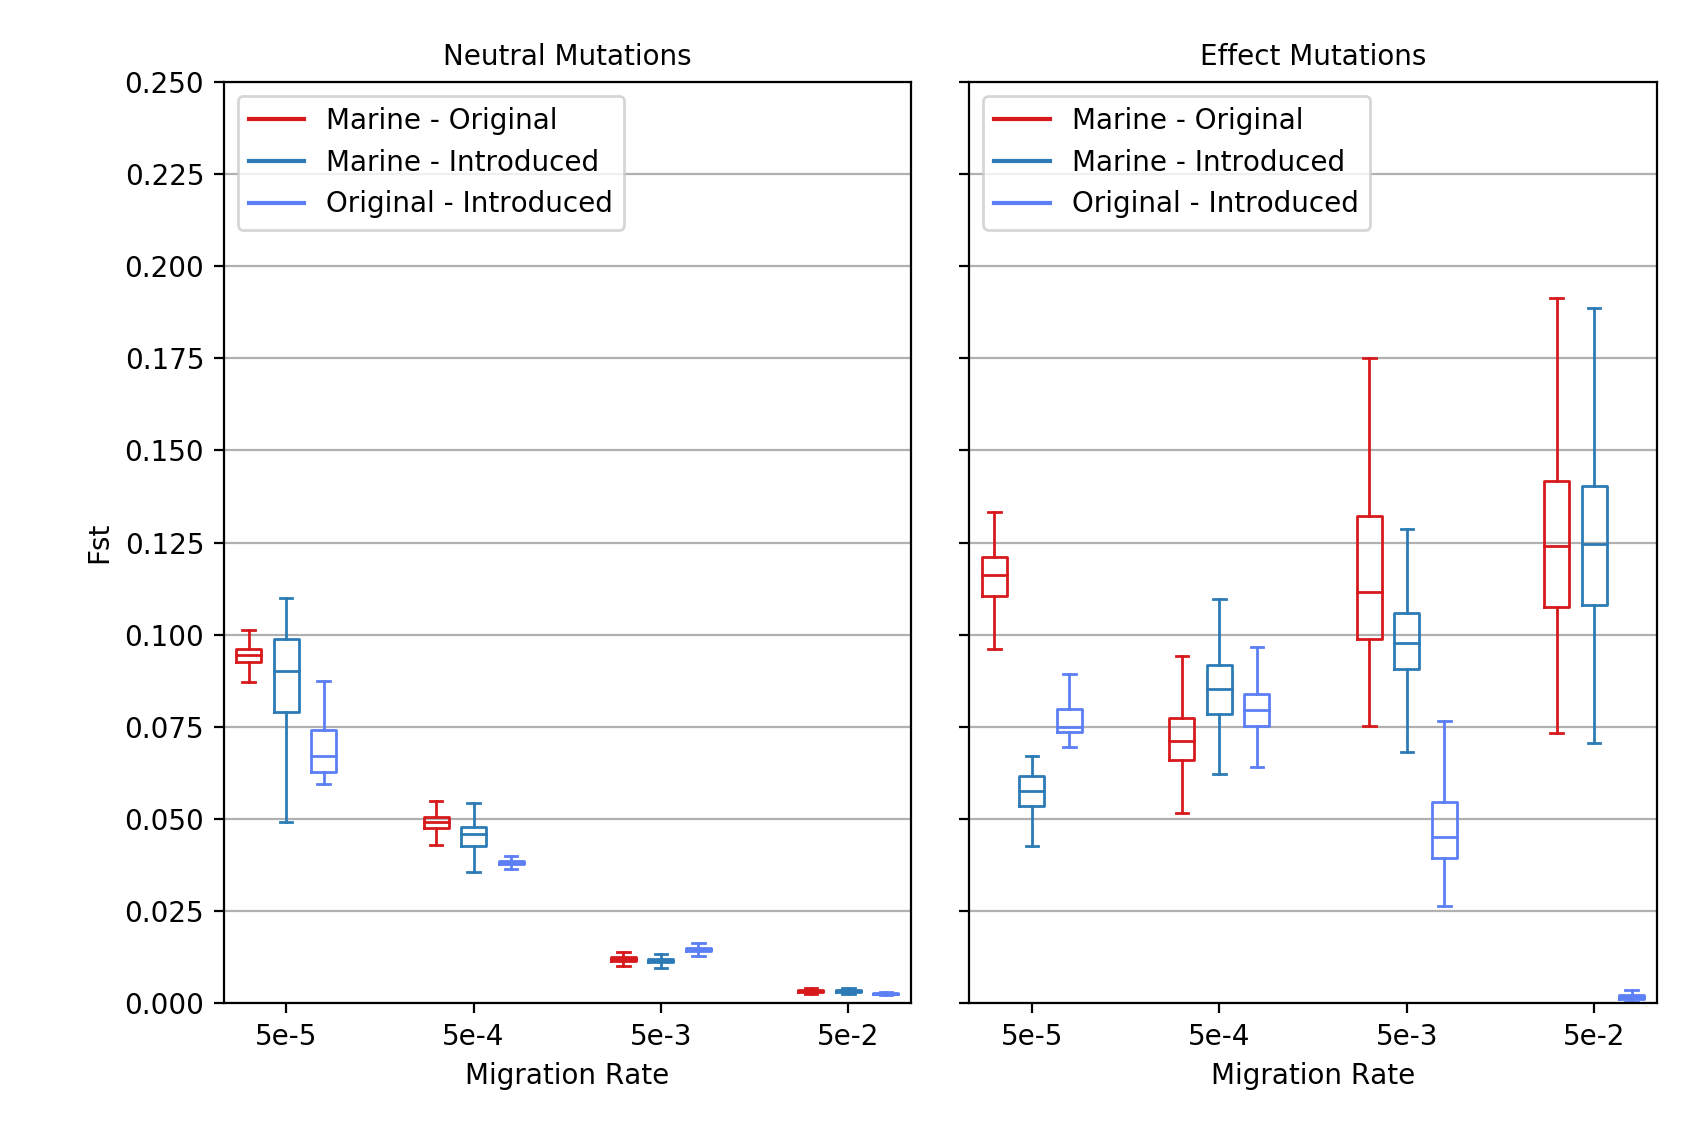
\includegraphics[width=0.8\linewidth]{matplotlibPlots/FST_HRR.png}
  		\caption{Distributions of $F_{st}$  values between the three subpopulations throughout the simulations.
		On the left, $F_{st}$ was calculated only on neutral mutation frequencies. On the right, $F_{st}$ was calculated
		only on effect (Impact on phenotype) mutation frequencies. 
		Effect mutations are acted upon by selection as they have an affect on fitness where neutral mutations  }
  		\label{fig:Fst}
	\end{center}
\end{figure}

Across increasing parameters of migration, we observed more gene flow across the populations. 
As can be seen in Figure \ref{fig:Fst},
$F_{st}$ values for neutral alleles steadily decline between all sets of populations as 
migration increases, this illustrates less difference between sections of the genome which are not acted up 
upon by selection, in all populations.
Additionally, standing genetic variance \todo{computed as?}
(seen in Figure \ref{fig:SGV})
values in the marine population steady increased with migration which suggests that more alleles from the 
lakes surrounding were exporting alleles into the marine individuals.
\todo{Something about SGV rates for the the other population}

%TIES TO NATURE?
%SPECIFICALLY (interesting stuff)

\subsubsection*{migration affects the speed of adaptation}

%FIGURES THAT SHOW THIS:
%-Time to adaptation
\begin{figure}
	\begin{center}
  		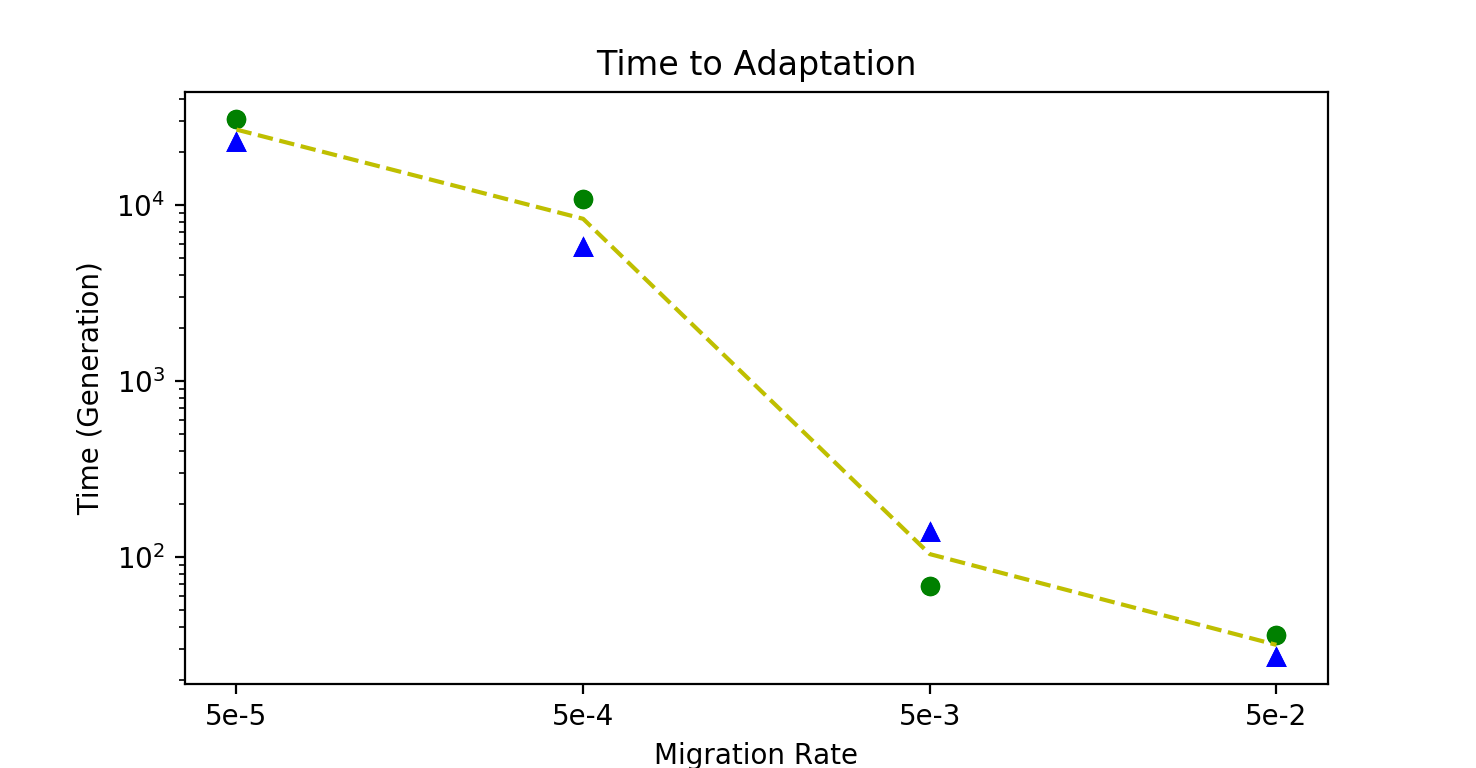
\includegraphics[width=0.8\linewidth]{matplotlibPlots/TimeToAdaptation.png}
  		\caption{Time to adaptation as a function of migration rate ($M$) parameter value. This is where we measure how many generation
		it takes for the introduced population's mean phenotype to come within 0.5 of the original lakes average phenotype. 
		Each point represents a simulation run at some value of $M$. 
		The yellow dashed line is the average of all points at each respective parameter value}
  		\label{fig:TimeToAdaptation}
	\end{center}
\end{figure}

We observed a dramatic shift in time until adaptation for the introduced populations
as migration rates increased. 
As can be seen in Figure \ref{fig:TimeToAdaptation} at the lowest migration rate of $5 * 10^{-5}$,
It took the introduced population over 20 thousand generations for the average phenotype of all the lakes to 
get to within 0.5 of the original lakes original phenotypes. 
\plr{From the plots it looks more like adaptation happens (at least in most lakes) by like 10K or 15K.}
This suggests that selection was acting primarily on new mutations, meaning the 
introduced lakes needed to wait for a beneficial mutation to arise before 
it was selected upon. 
\plr{We should do the calculation to see if this makes sense: 
    there's one new effect mutation in the right direction every 100 generations in the lakes,
    one of effect size $s$ has probability of about $s/2$ of not being lost to drift...}
There was a positive correlation between the amount of standing genetic variation in the 
marine and the rapid adaptation of the introduced populations.

%TIES TO NATURE?
 
\subsubsection*{sharing of freshwater adapted alleles}

%FIGURES THAT SHOW THIS:
%-MPAA / IND
%-Total/Avg shared
\begin{figure}
	\begin{center}
  		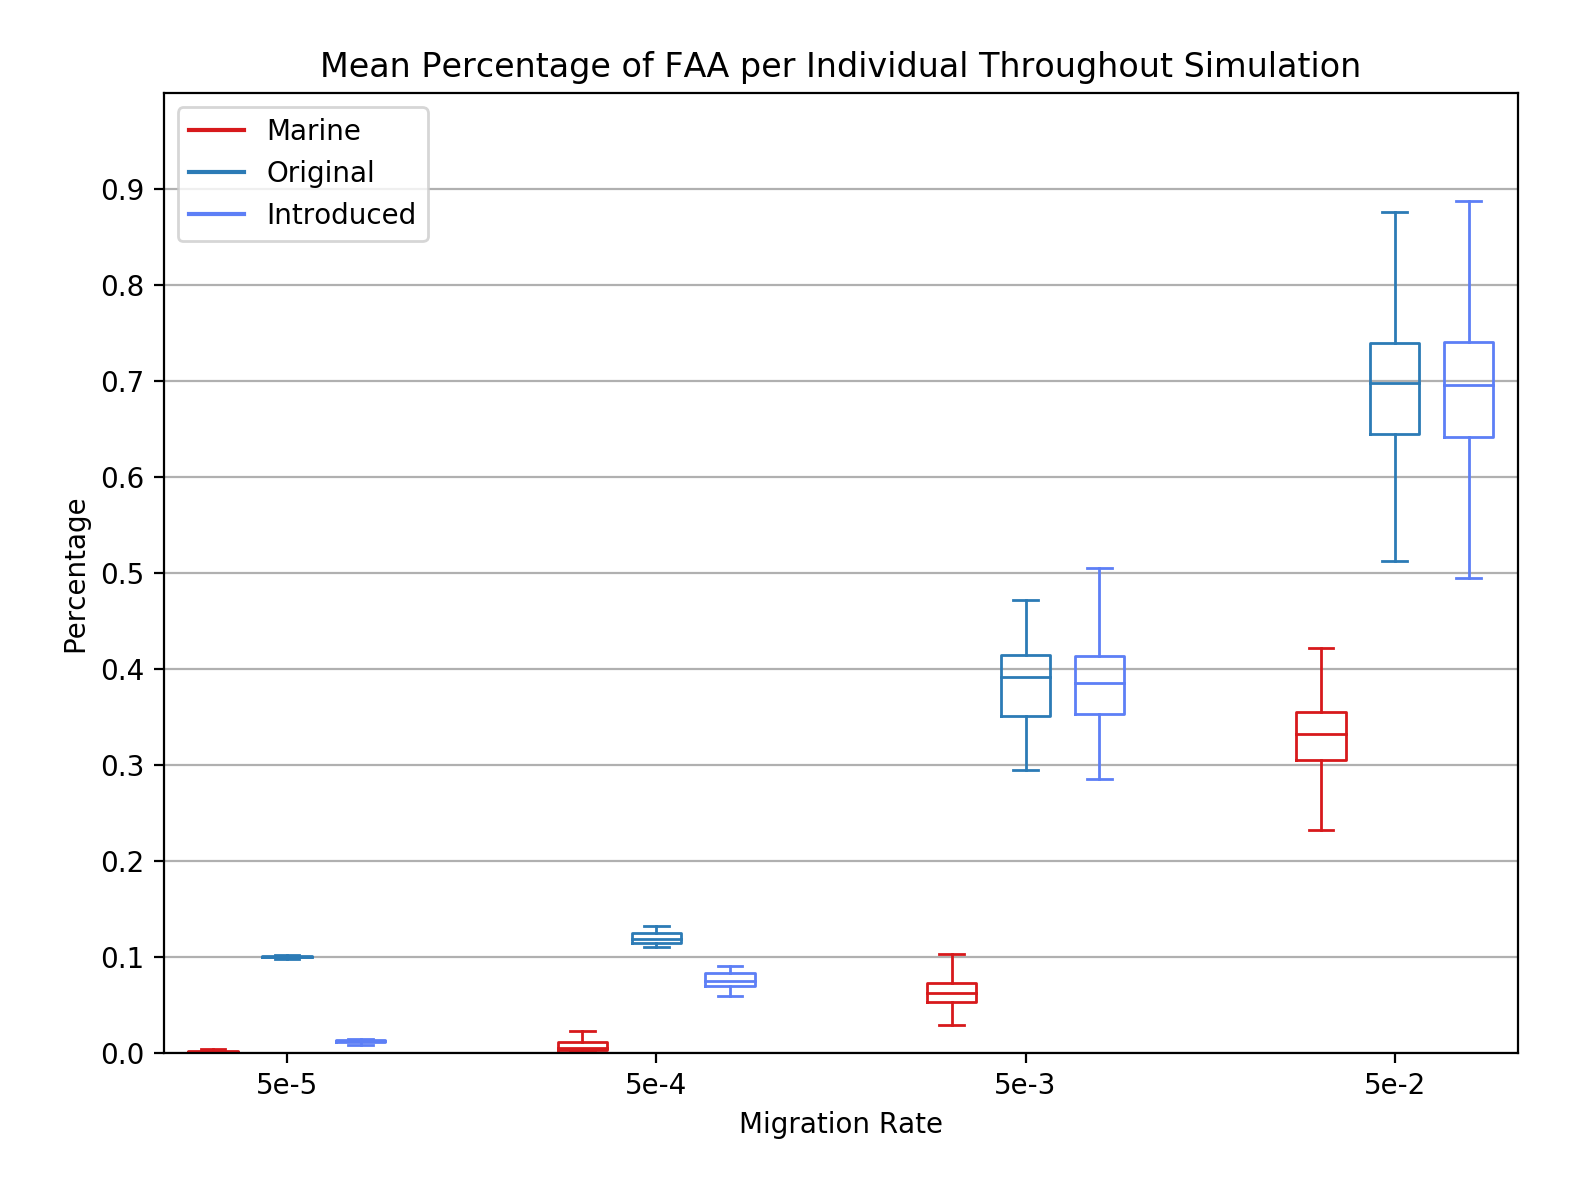
\includegraphics[width=\linewidth]{matplotlibPlots/MPFAI.png}
  		\caption{Distributions of mean percentage of freshwater adapted alleles (FAA) per individual throughout the simulation run, for each subpopulation.
		We count the total number of freshwater alleles for each individual before averaging them in each population and dividing by the total number of defined
		freshwater adapted alleles.
		Looking at total number of FAA per individual gives us an idea behind how many alleles underly a freshwater haplotype, 
		while the percentage tells us the variance of the haplotype}
		\label{fig:MPFAI}
	\end{center}
\end{figure}

\begin{figure}
	\begin{center}
  		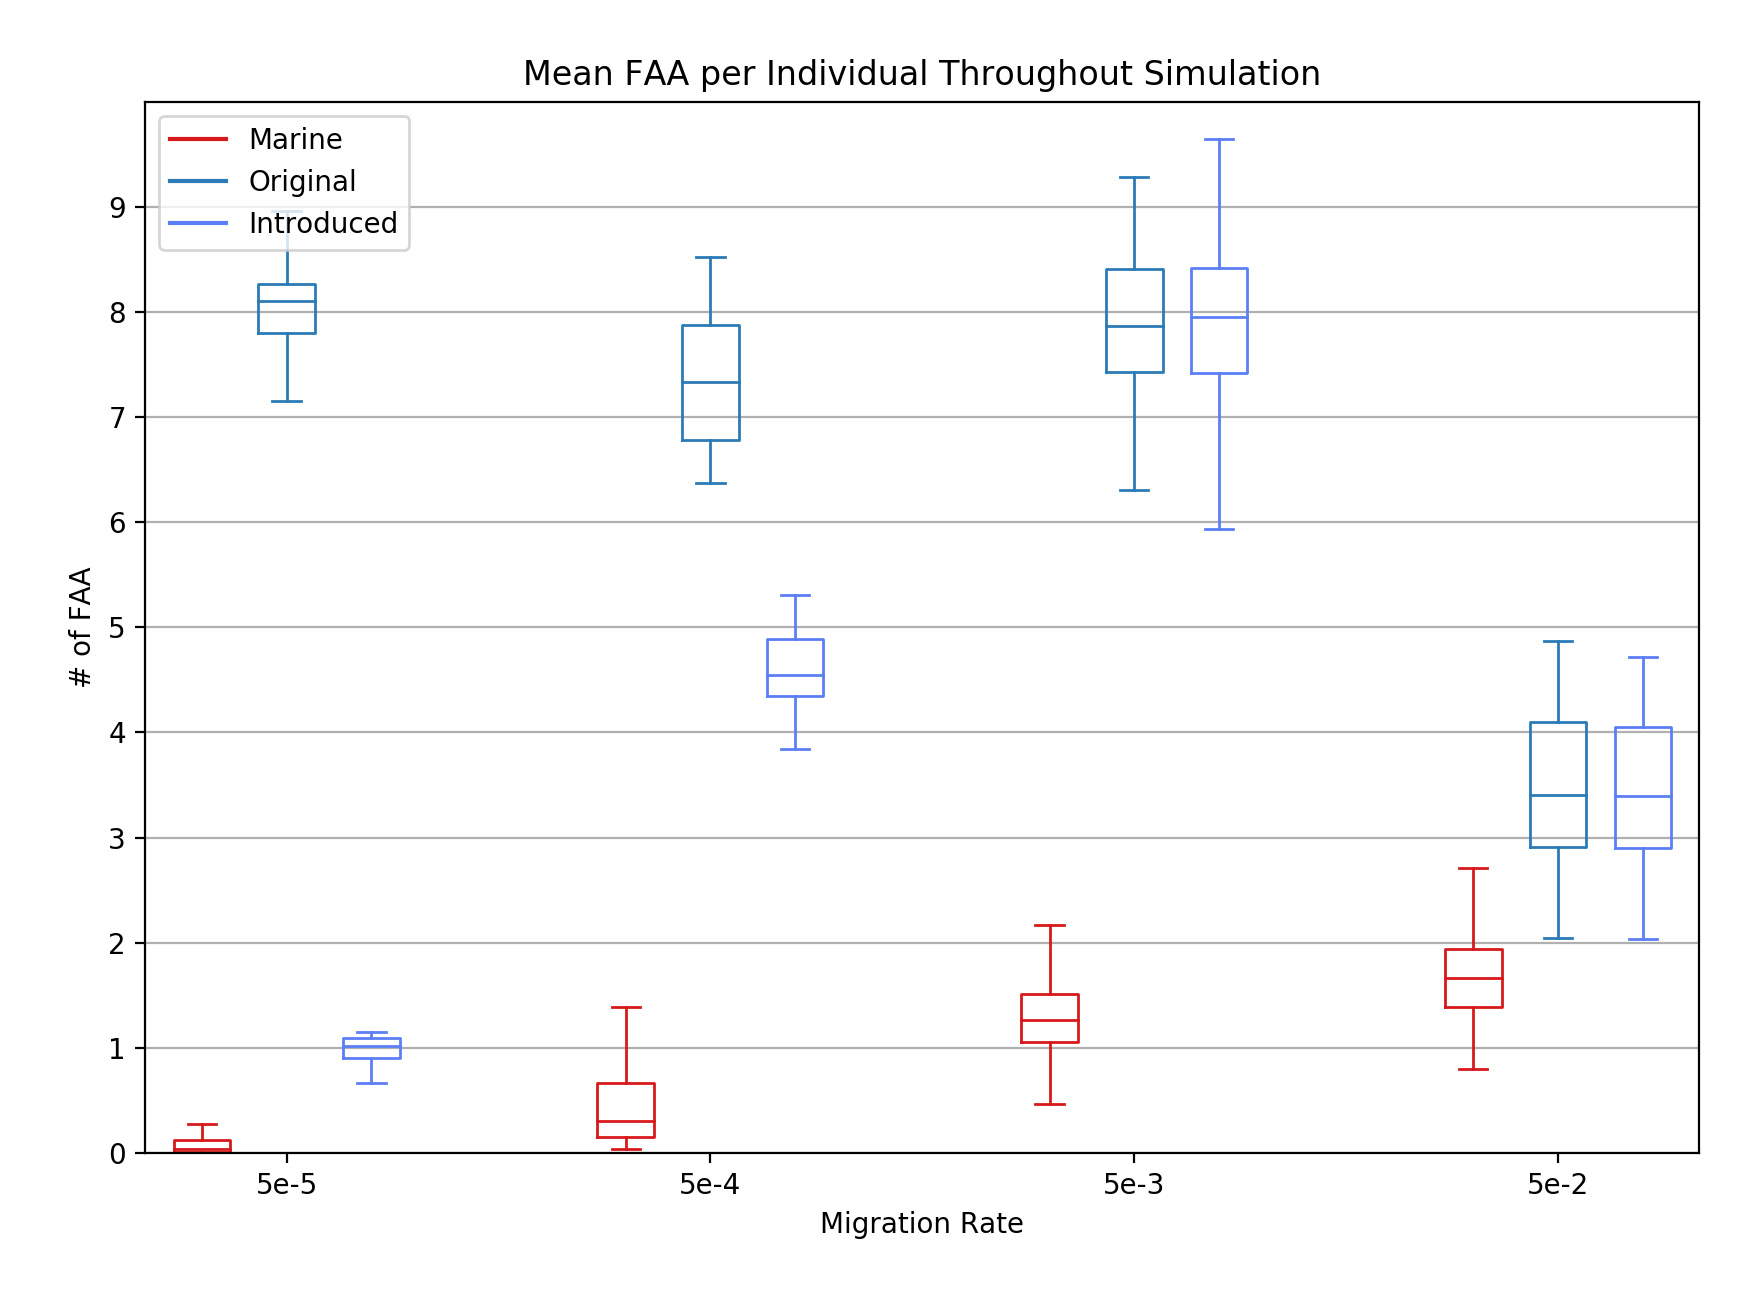
\includegraphics[width=\linewidth]{matplotlibPlots/MFAI.png}
  		\caption{Distributions of mean number of freshwater adapted alleles (FAA) per individual throughout the simulation run, for each subpopulation.
		We count the total number of freshwater alleles for each individual before averaging them in each population and dividing by the total number of defined
		freshwater adapted alleles.
		Looking at total number of FAA per individual gives us an idea behind how many alleles underly a freshwater haplotype, 
		}
  		\label{fig:MNFAI}
	\end{center}
\end{figure}

\begin{figure}
	\begin{center}
  		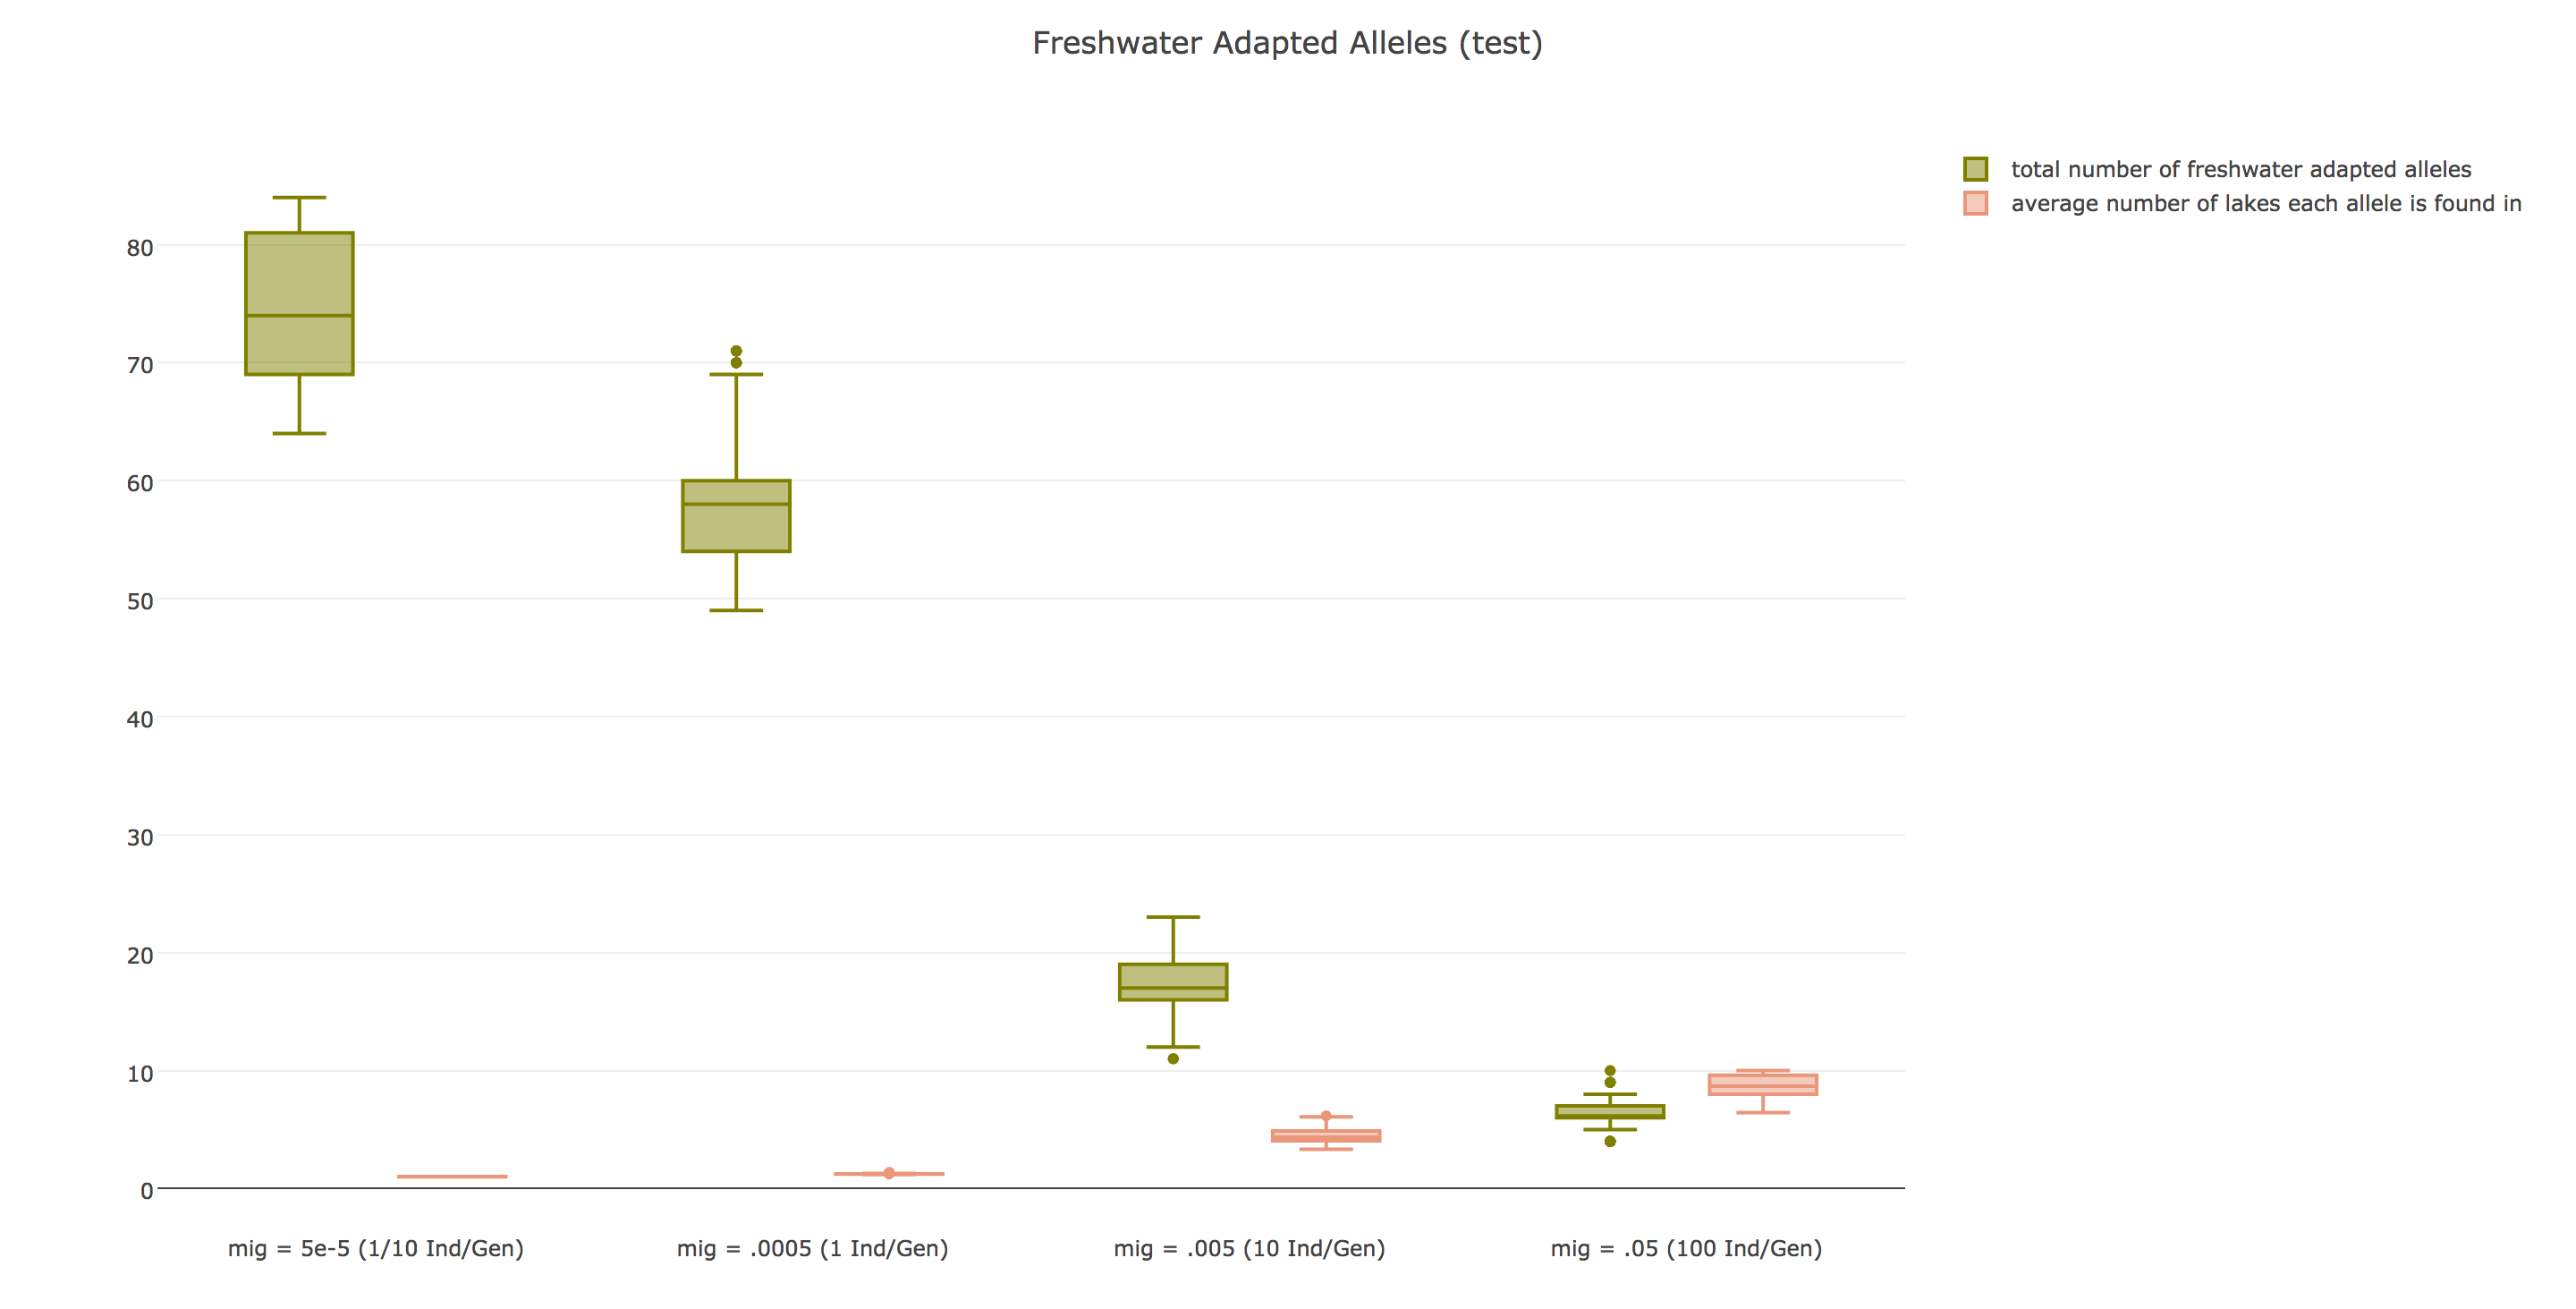
\includegraphics[width=\linewidth]{plotlyPlots/NumFAA.png}
  		\caption{(PLACEHOLDER)}
		\label{fig:NumFAA}
	\end{center}
\end{figure}

\begin{figure}
	\begin{center}
  		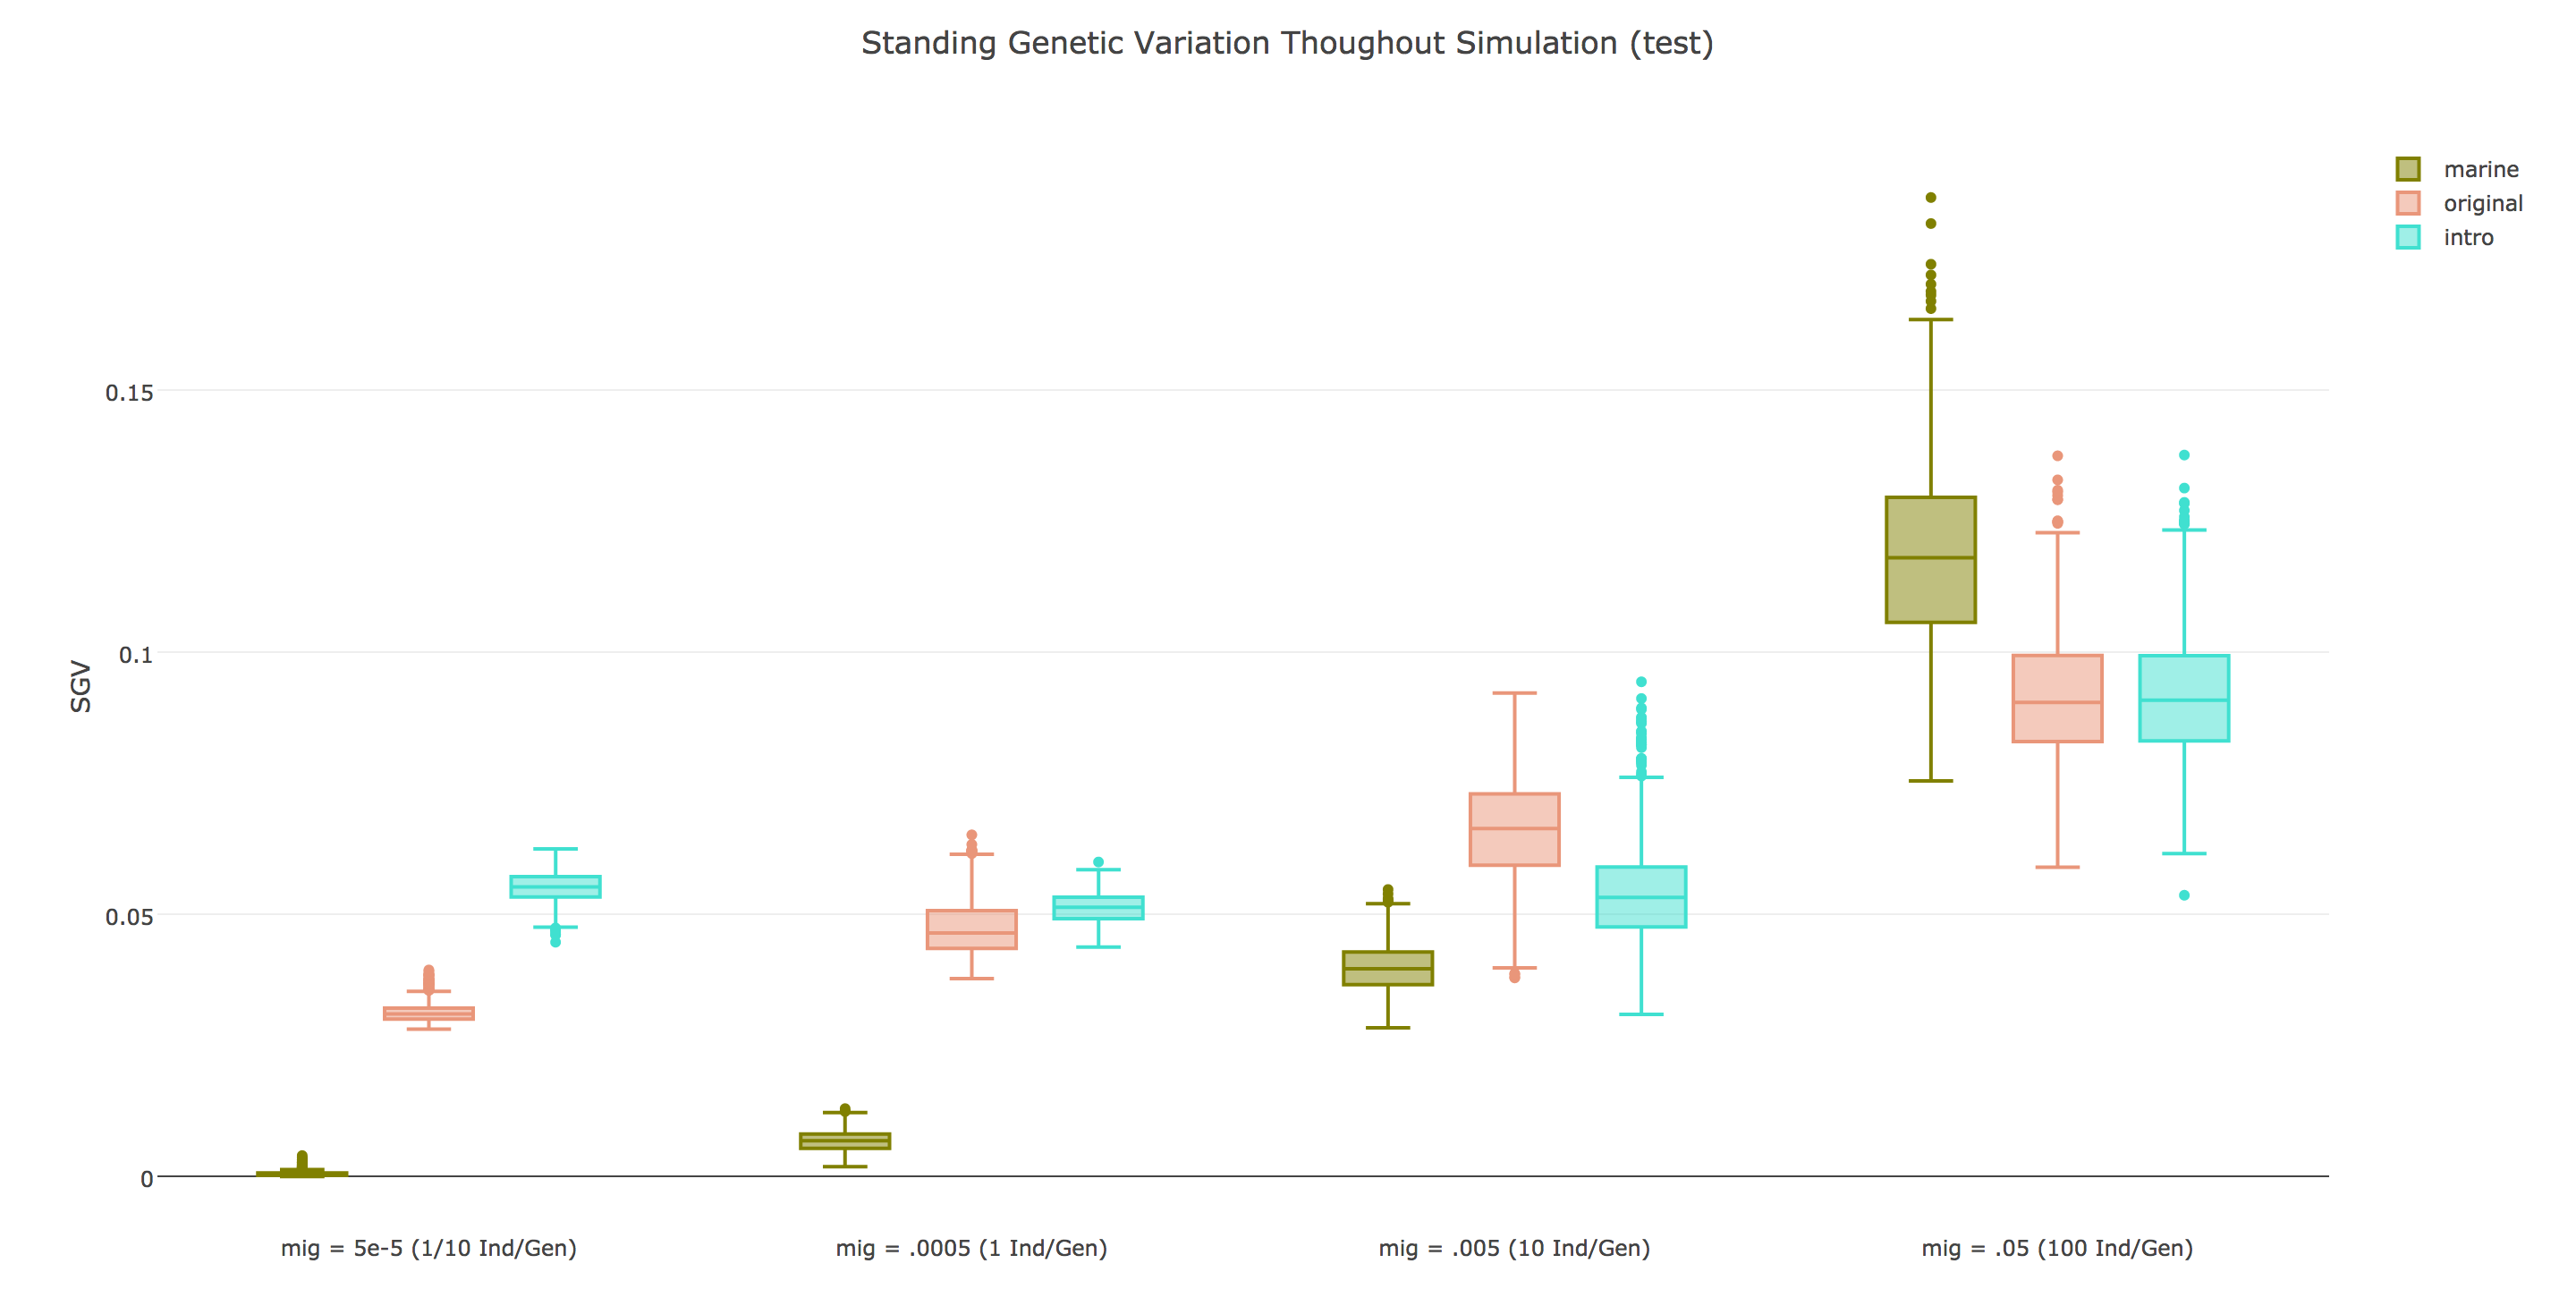
\includegraphics[width=\linewidth]{plotlyPlots/StandingGeneticVariation.png}
  		\caption{(PLACEHOLDER)}
		\label{fig:SGV}
	\end{center}
\end{figure}



To further investigate this correlation, we take a look at the FAA driving 
local adaptation of the introduced population. 
One common metric we investigate is the percentage of FAA per individual in each of the populations. 
This gives us a general look at the where these alleles are being distributed. 
Looking at the lowest migration rate for the original lakes population In Figure (MPAA / IND) 
We see that the average individual has almost exactly $1/10^{th}$ of the total defined FWAA throughout the simulation. 
Because FAA are defined among \textit{any} population, this suggests that each one of the $10$ 
lakes has created their own solution to adaptation of the the freshwater selective pressure. 

As we can see in Figure (Total/Avg shared)
as migration rate parameter increases for the simulations, 
we see the distribution of the total number of FAA's decrease, and 
the average number of lakes each allele appears in at high frequency ($p > 0.5$), increase.
With the distribution of effect size remaining the same across all simulations, 
these are both suggestive of the original lakes sharing solutions to the same selective pressure.

%TIES TO NATURE?

%SPECIFICALLY (interesting stuff)

\subsubsection*{We see Migration Load after a certain threshold of migration}

%FIGURES THAT SHOW THIS:
%- Phenotype Distribution
\begin{figure}[h!tb]
	\begin{center}
  		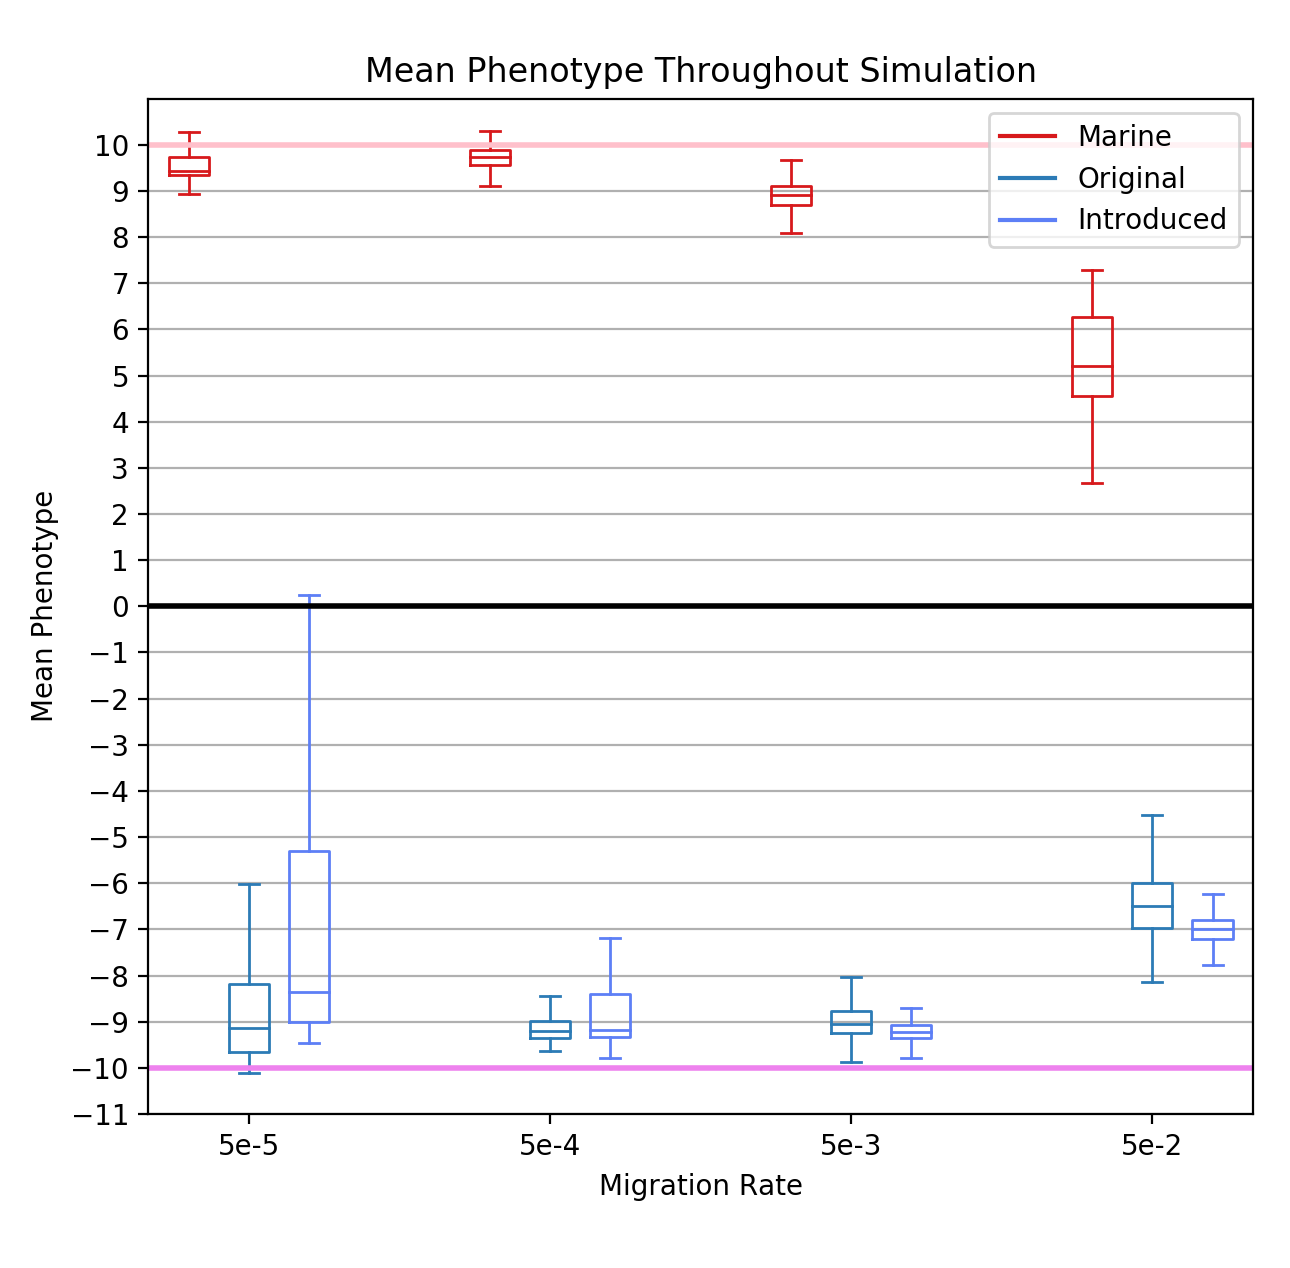
\includegraphics[width=0.6\linewidth]{matplotlibPlots/MeanPhenotype1.png}
  		\caption{Distribution of mean phenotype throughout simulation runs at separate migration rate ($M$) parameter values, for each population.
		The dashed pink line (Pheno = +10) is the optimum phenotype any individual in the marine environment.
		In contrast the purple line at (Pheno = -10) represents the optimum for any individual in the freshwater environment. 
		All individuals at generation 0 (beginning of the simulation) 
		}
  		\label{fig:MeanPhenotype}
	\end{center}
\end{figure}

%GENERAL

In the distributions we have shown across migration rate parameter values, 
We have experienced the most dramatic shifts of the population dynamics at $M = 5x10^{-3}$.
After a threshold between this and $M = 5x10^{-2}$, we start to experience migration load. 
Significant gene flow constricts local adaptation
as a consequence of a large number of offspring through hybridization events between subpopulations.
In Figure \ref{fig:MeanPhenotype} at $M = 5x10^{-2}$, we can see the distribution of average phenotype throughout the simulation
pull towards the opposing selective pressure value and away from the local optimum in all subpopulations.




%TIES TO NATURE?

%SPECIFICALLY (interesting stuff)
	
\subsubsection*{There is a Qualitative Threshold of migration rates}

%FIGURES THAT SHOW THIS:
%all
%TIES TO NATURE?
%SPECIFICALLY (interesting stuff)

%GENERAL
We have found that too little migration leads to selection upon new mutations in all subpopulations and lakes alike. 
In contrast, at high migration rates we have seen that migration load limits 
the ability for species to locally adapt to the selective pressure of their environment.
This leads us to consider a window (Goldilocks Zone) of introgression which allows for the transportation
of FAA's without migration load. In a species that commonly is subjected to two general types of selective pressure 
such as marine and 
\plr{Maybe this goes in the Discussion? Remaining observations could merge with the previous section.}


\subsection{Genomic Architecture}

\begin{figure}
	\begin{center}
  		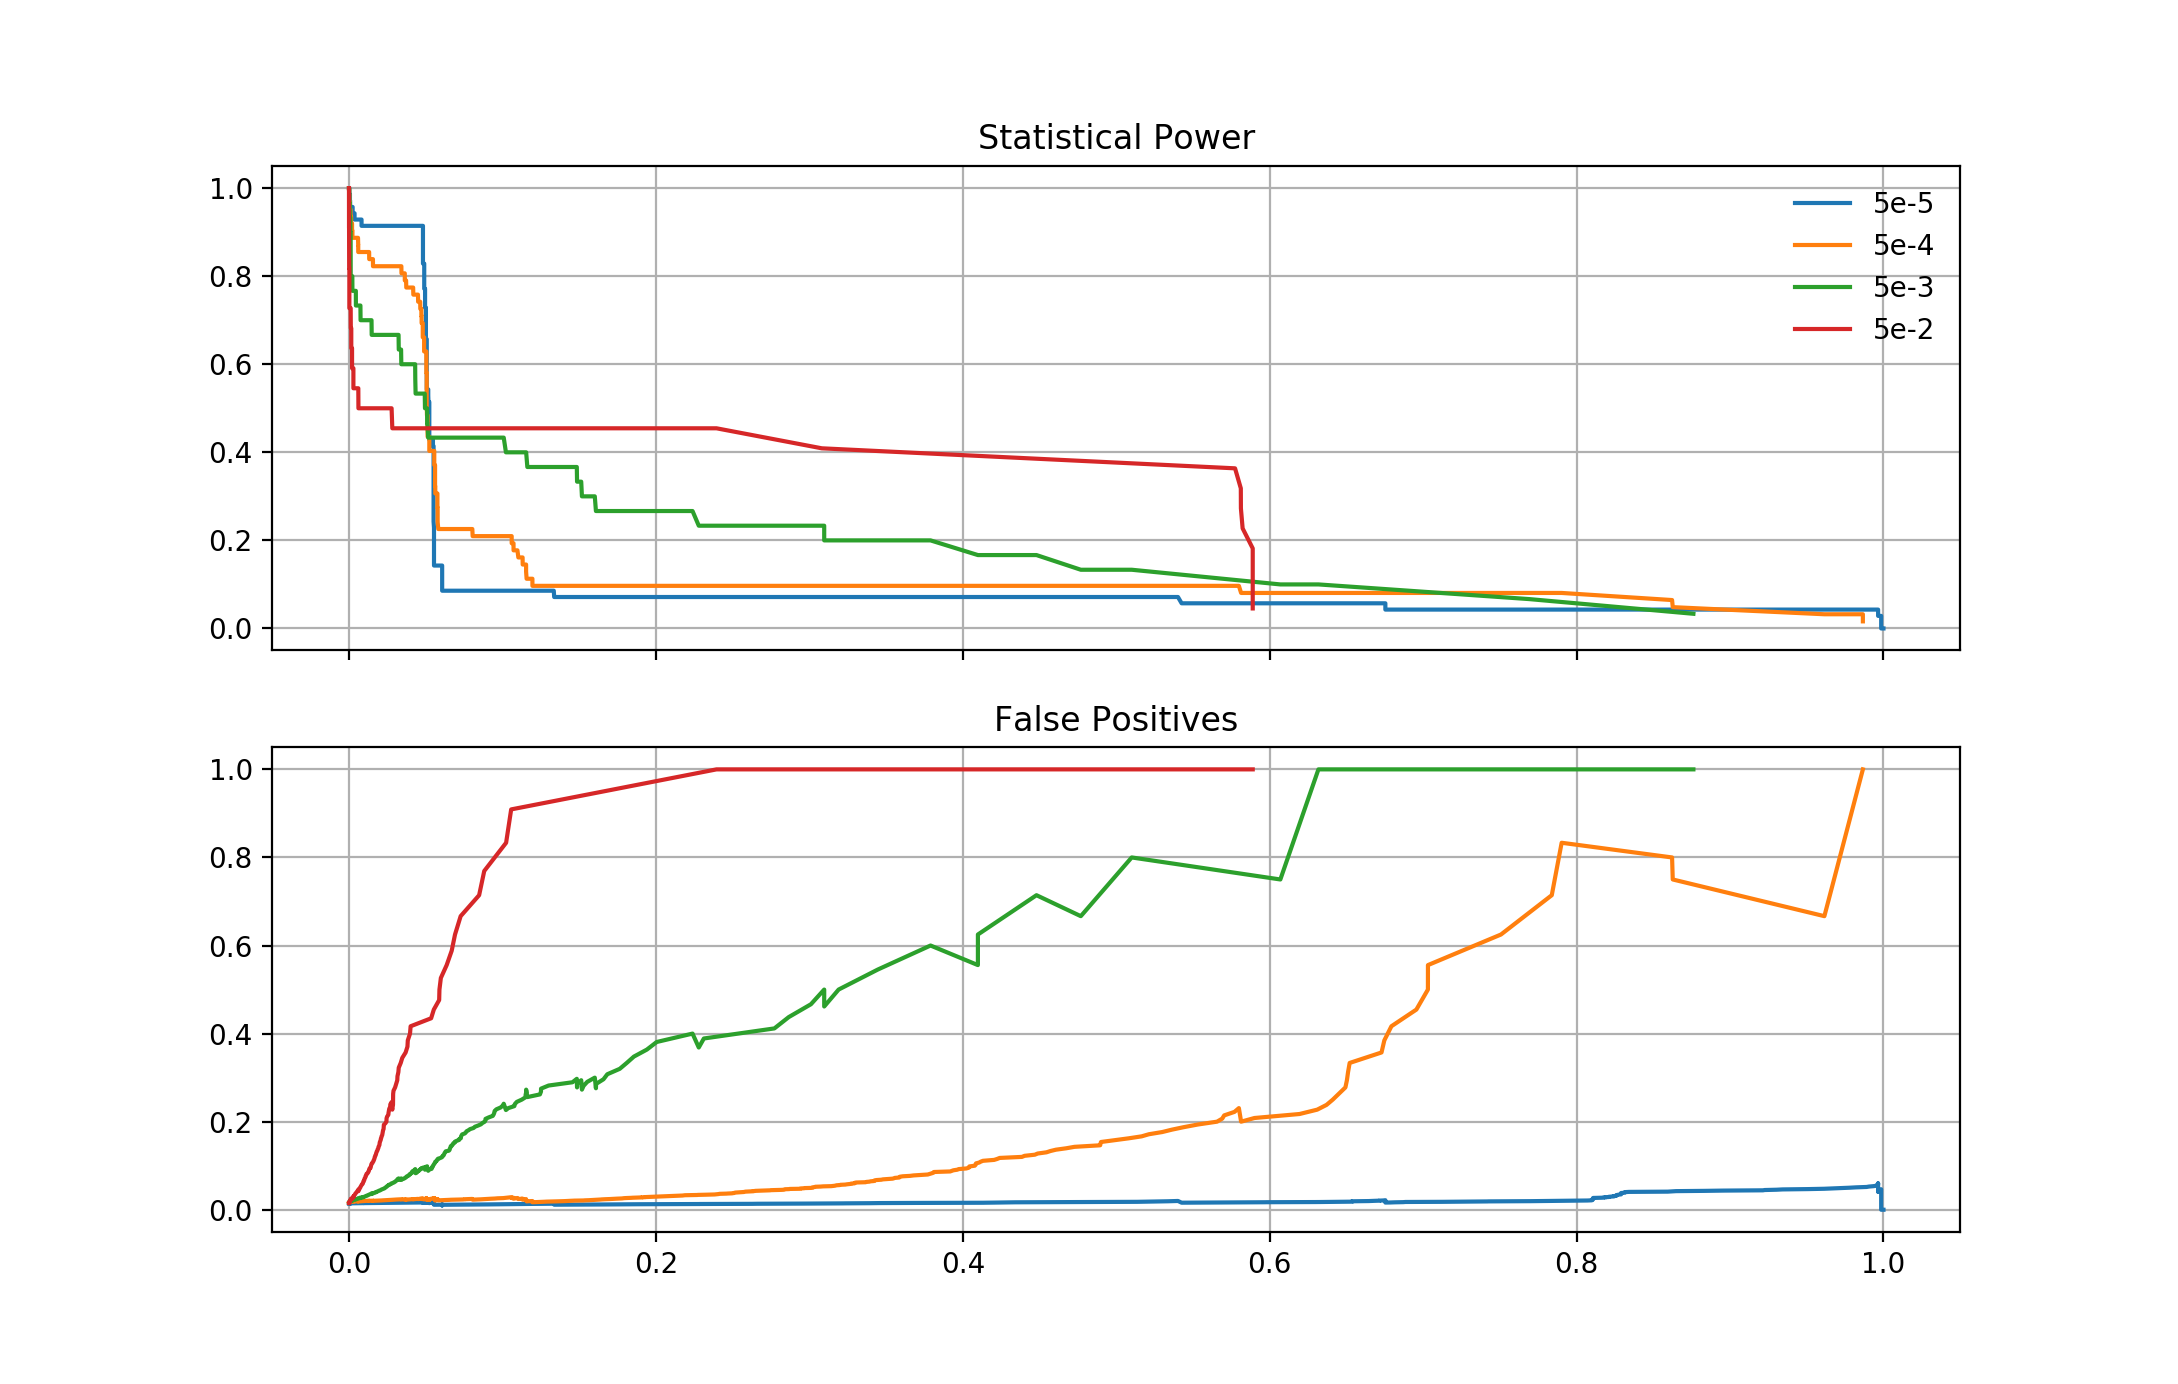
\includegraphics[width=0.7\linewidth]{matplotlibPlots/Power_FP.png}
  		\caption{ 
		%SP - suppose you have an Fst Peak, how likely is it that that region is causal. 
		Statistical Power and False Positives as a function of $F_{st}$ threshold. 
		Statistical Power is the likelihood that a SNP will be predicted to have an effect on phenotype when there is an effect to be detected (?).
		False Positives give us the ratio of SNPs that effect phenotype to total SNPs greater than the $F_{st}$ threshold.
		}
  		\label{fig:Power_FP}
	\end{center}
\end{figure}

%Suppose you have a Fst Peak, ___ how likely is it that that region is causal. and conversely, what proportion of 
%the causal loci are under Fst Peaks.

%

Here, we take a closer look at the genomic architecture of local adaptation between freshwater and marine individuals. 
Often when looking at real datas, biologists observe patterns of $F_{st}$ and clustering of alleles that suggest causative loci for certain traits.
However, researchers would like to know how parameters such as migration and recombination impact the results from natural populations.
To give an idea about the impact of these parameters in our model, we examine the distribution, location, and false positive rate on predicting effect loci
given the $F_{st}$ per SNP across the genome. 


\subsubsection*{False-Positives \& Statistical Power}

\plr{Start off by talking about Fst along the genome, then say ``if we identify QTL as the outliers, then...''}
\plr{I vote for combining and including figures \ref{fig:Fst2} and \ref{fig:Fst3}.}
Given that migration increases the gene flow between subpopulations, how valid are $F_{st}$ peaks at different $M$. 
Knowing exactly which mutations effect phenotype in our simulations, 
we can look at the statistical power and false positives given $F_{st}$ per SNP across the genome. 
In Figure \ref{fig:Power_FP} , looking at an $F_{st}$ threshold greater than 1, we see the two lowest migration rates $10^{-5}$ and $10^{-4}$ having very little statical power. 
This along with low false positive rate across all $F_{st}$ threshold values is fairly predictable when you consider the high $F_{st}$ values across the genome. 

%The lowest migration rate of $10^{-5}$ also has a very low false positive rate across all $F_{st}$ threshold values.






%\subsubsection*{Low Recombination Causes Clustering}
\begin{comment}
\begin{figure}[h!tb]
	\begin{center}
  		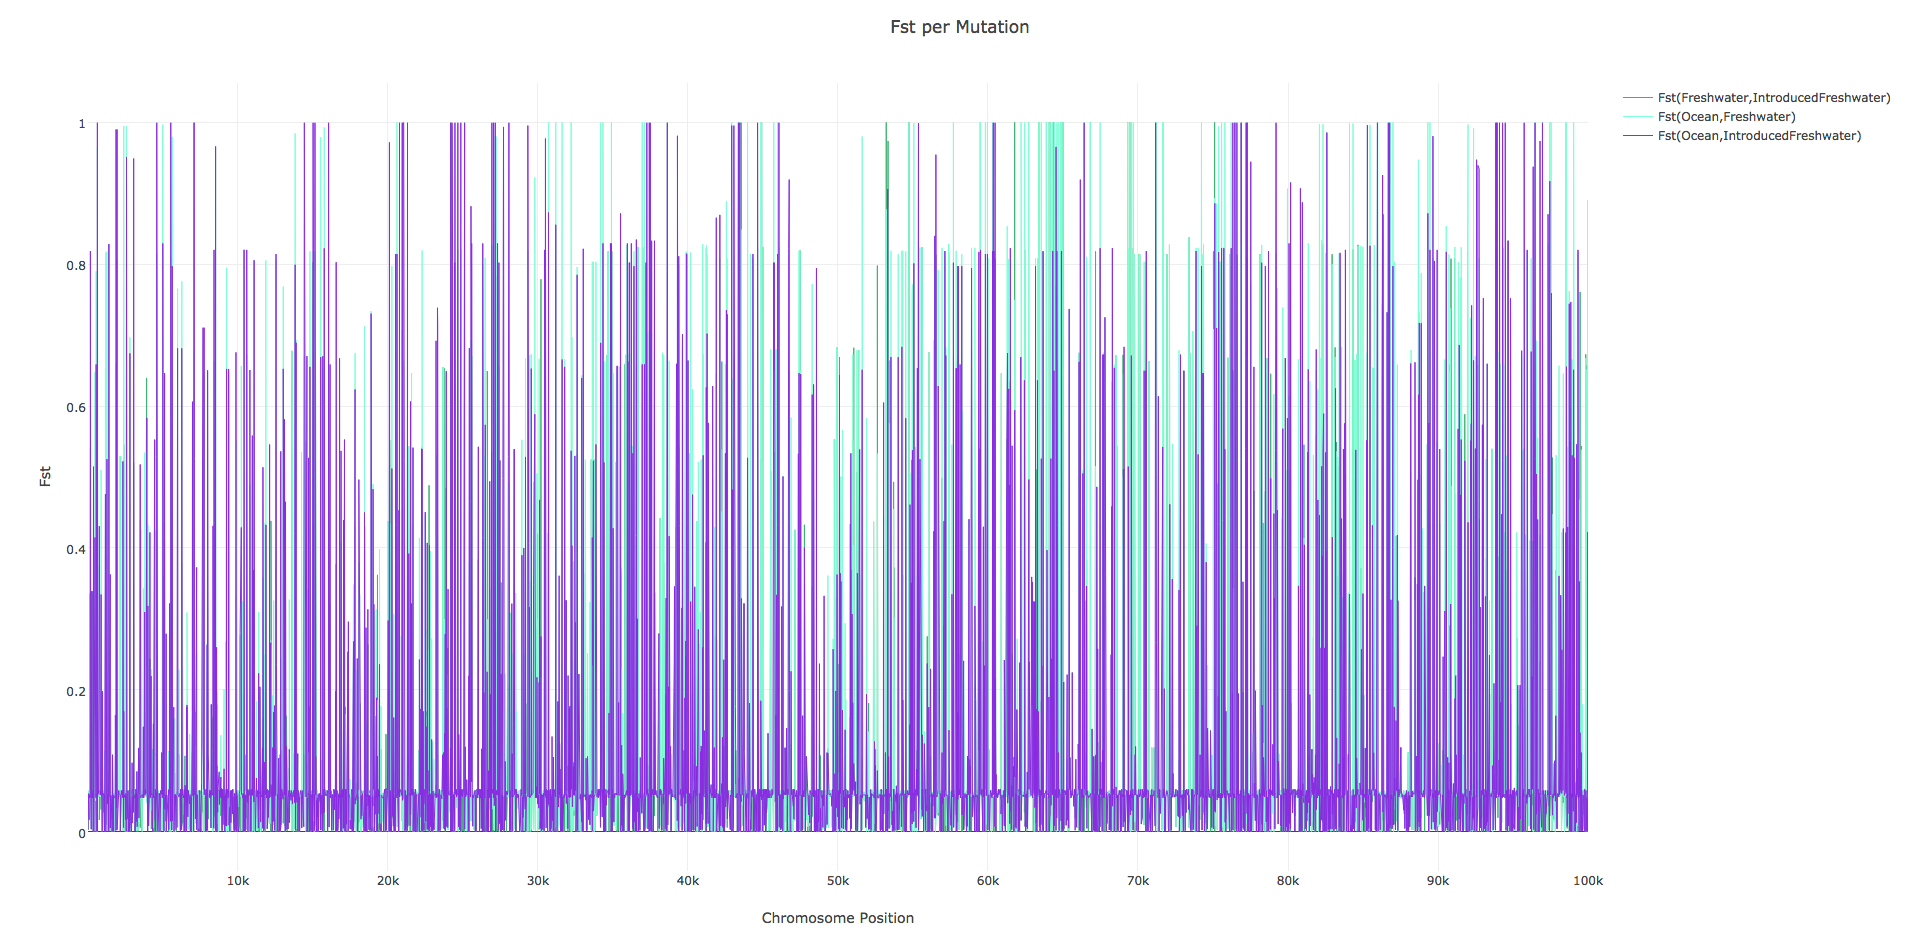
\includegraphics[width=0.7\linewidth]{plotlyPlots/FstAcross5e-5.png}
  		\caption{ (PLACEHOLDER)
		}
  		\label{fig:Fst1}
	\end{center}
\end{figure}

\begin{figure}[h!tb]
	\begin{center}
  		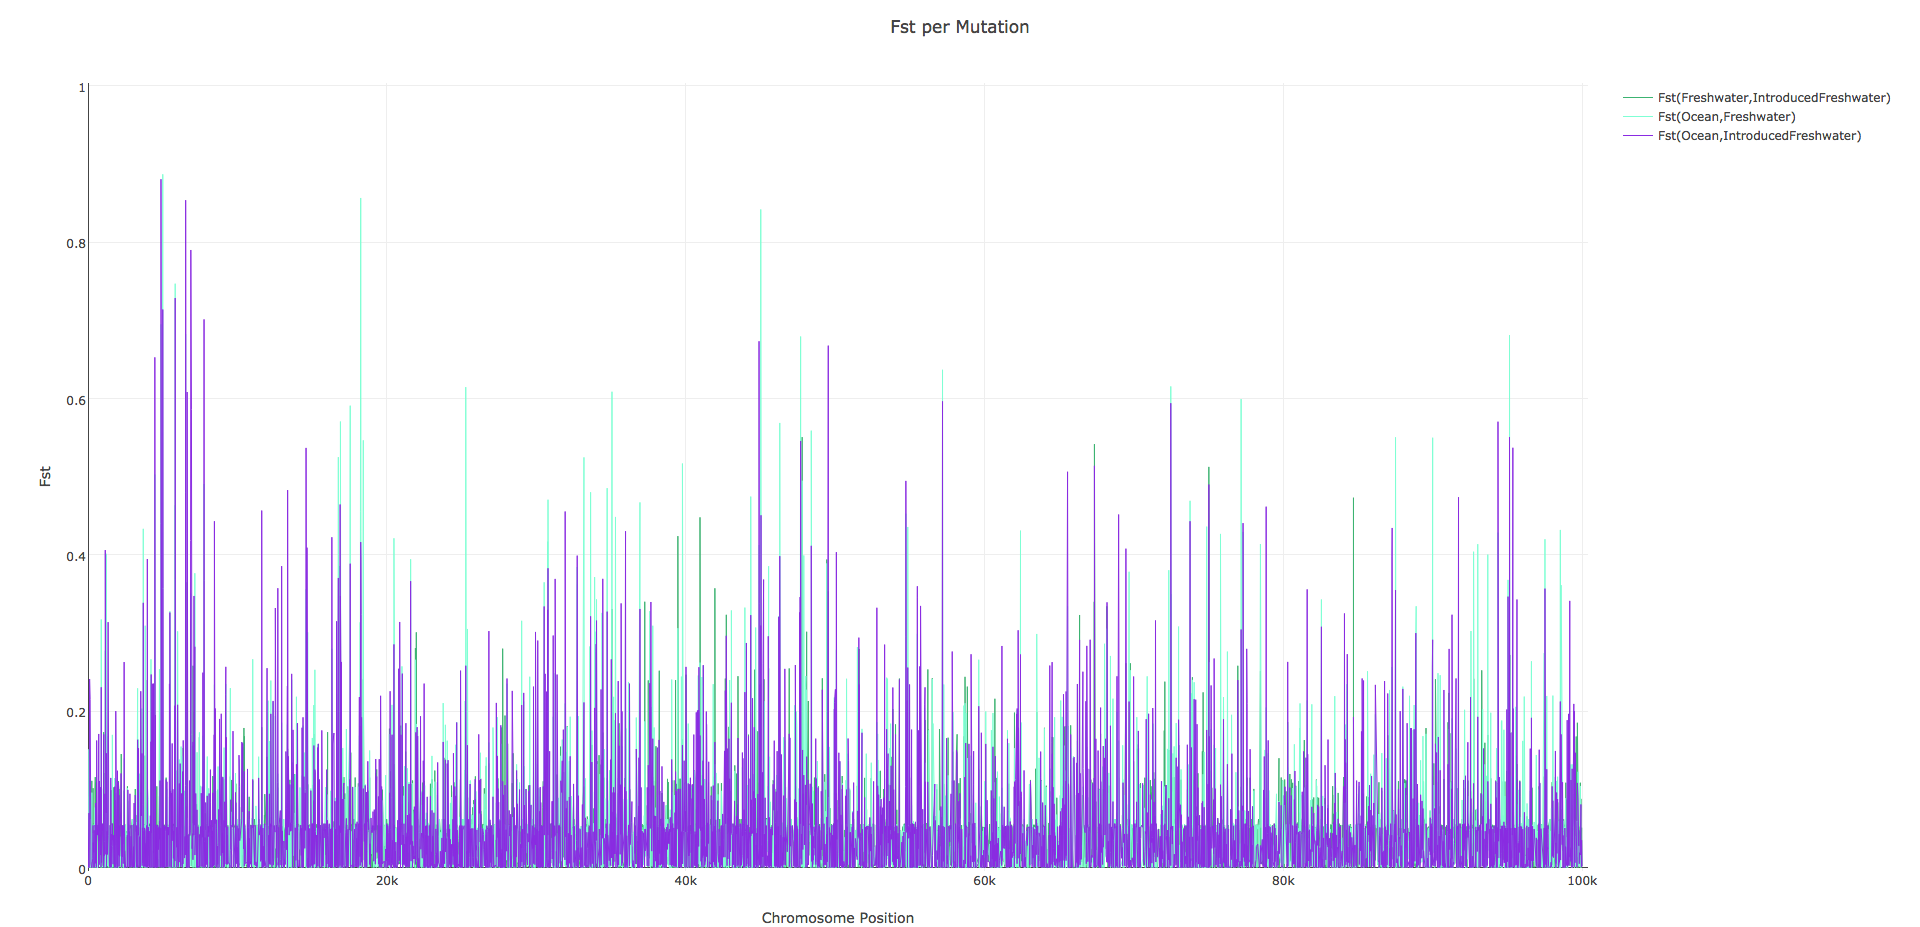
\includegraphics[width=0.7\linewidth]{plotlyPlots/FstAcross5e-4.png}
  		\caption{(PLACEHOLDER)
		}
  		\label{fig:Fst2}
	\end{center}
\end{figure}

\begin{figure}[h!tb]
	\begin{center}
  		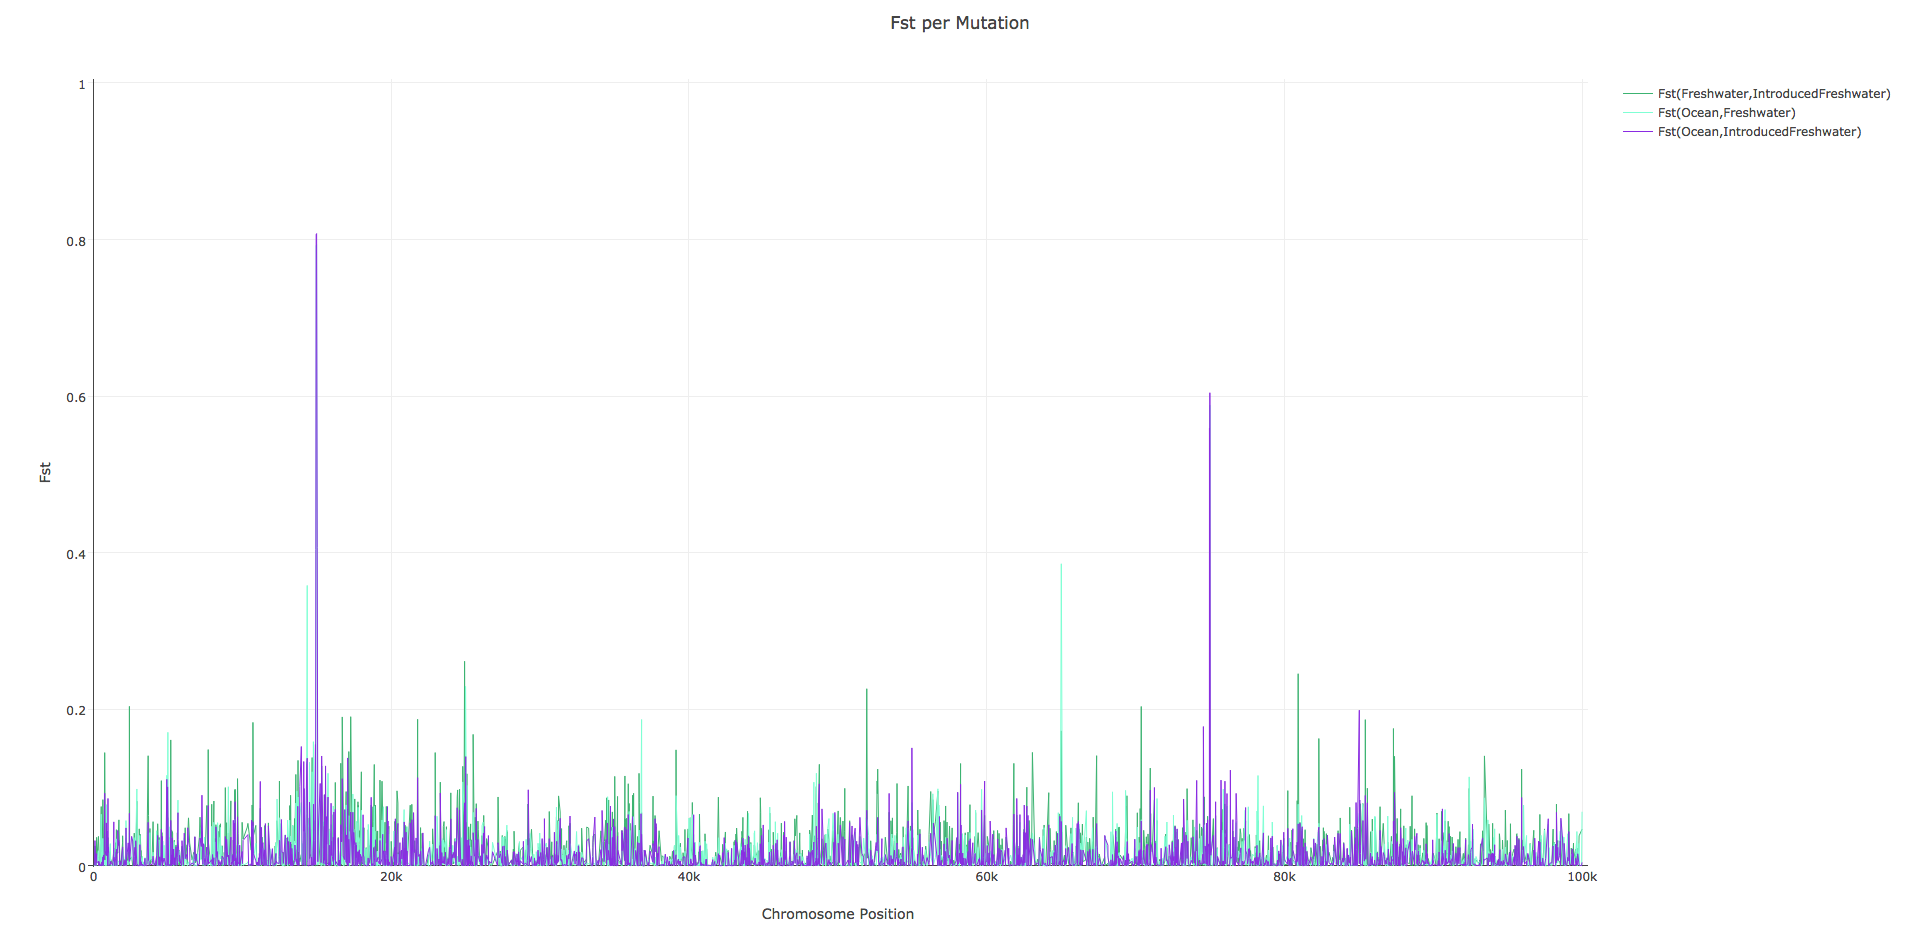
\includegraphics[width=0.7\linewidth]{plotlyPlots/FstAcross5e-3.png}
  		\caption{(PLACEHOLDER)
		}
  		\label{fig:Fst3}
	\end{center}
\end{figure}

\begin{figure}[h!tb]
	\begin{center}
  		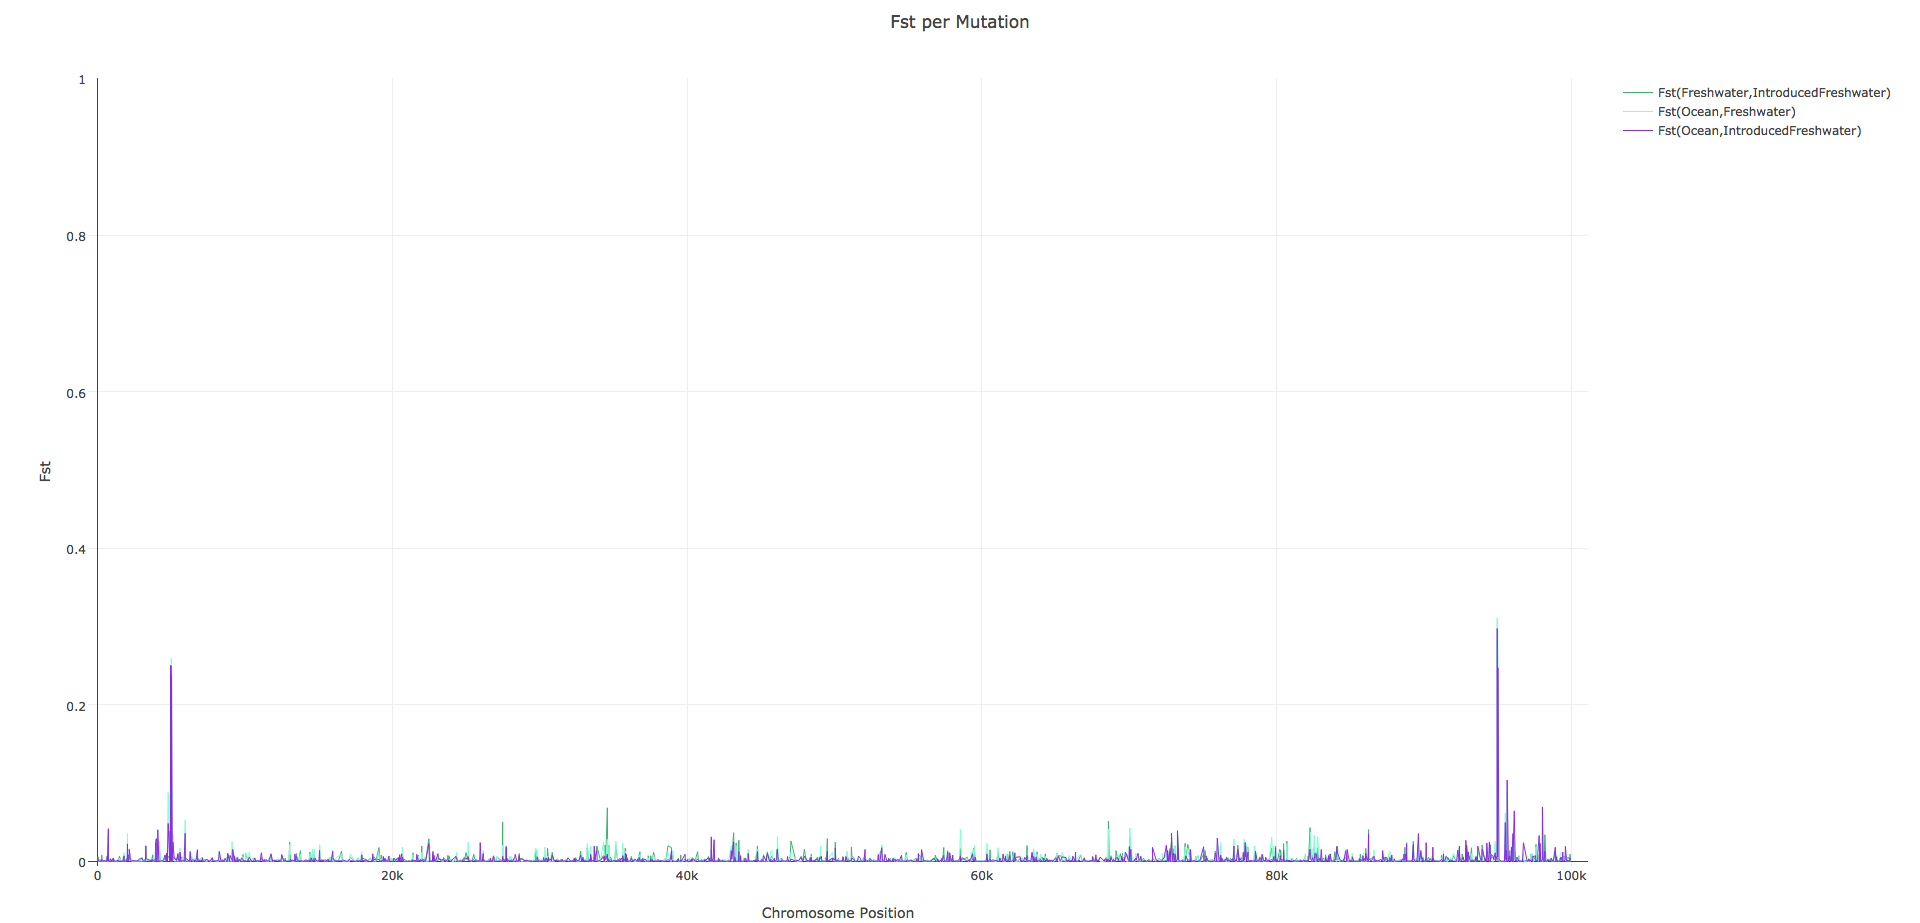
\includegraphics[width=0.7\linewidth]{plotlyPlots/FstAcross5e-2.png}
  		\caption{(PLACEHOLDER)
		}
  		\label{fig:Fst4}
	\end{center}
\end{figure}

\begin{figure}[h!tb]
	\begin{center}
  		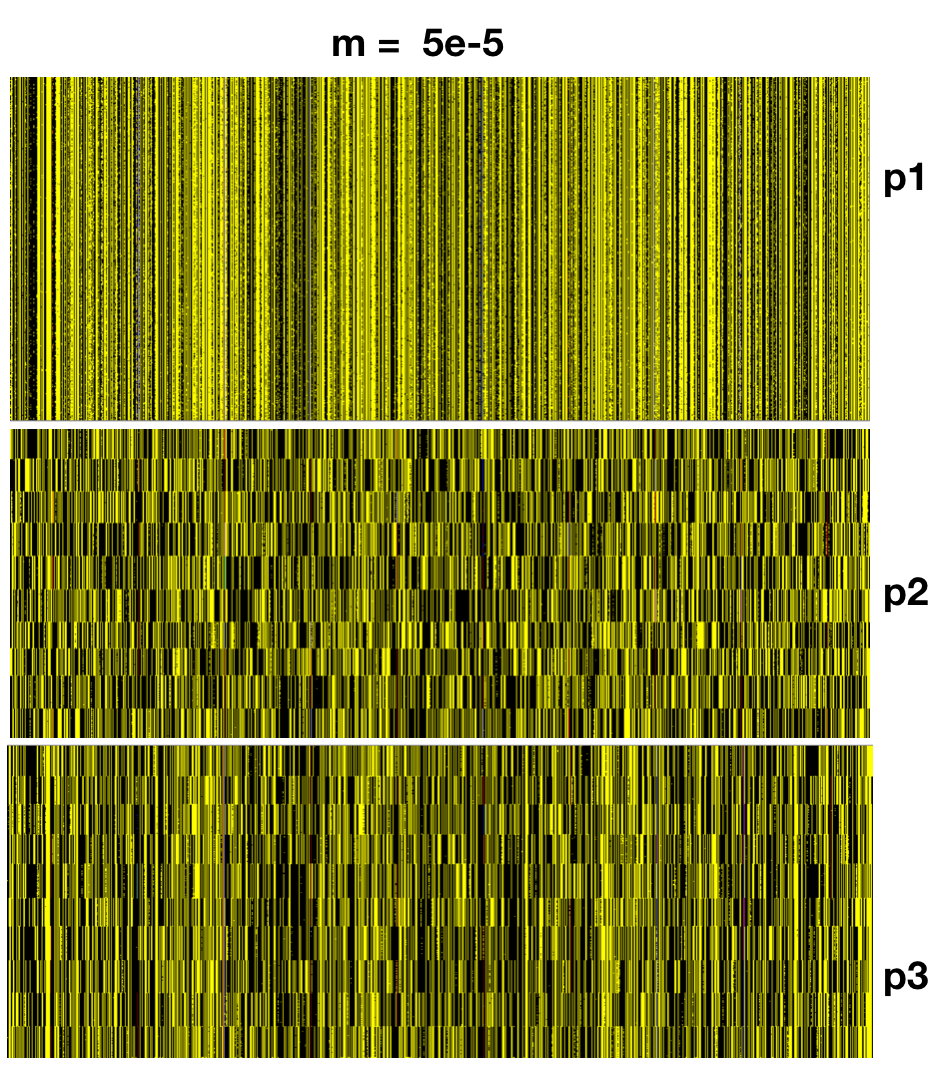
\includegraphics[width=0.7\linewidth]{plotlyPlots/Haplo5e-5.png}
  		\caption{ (PLACEHOLDER)
		}
  		\label{fig:Haplo1}
	\end{center}
\end{figure}

\begin{figure}[h!tb]
	\begin{center}
  		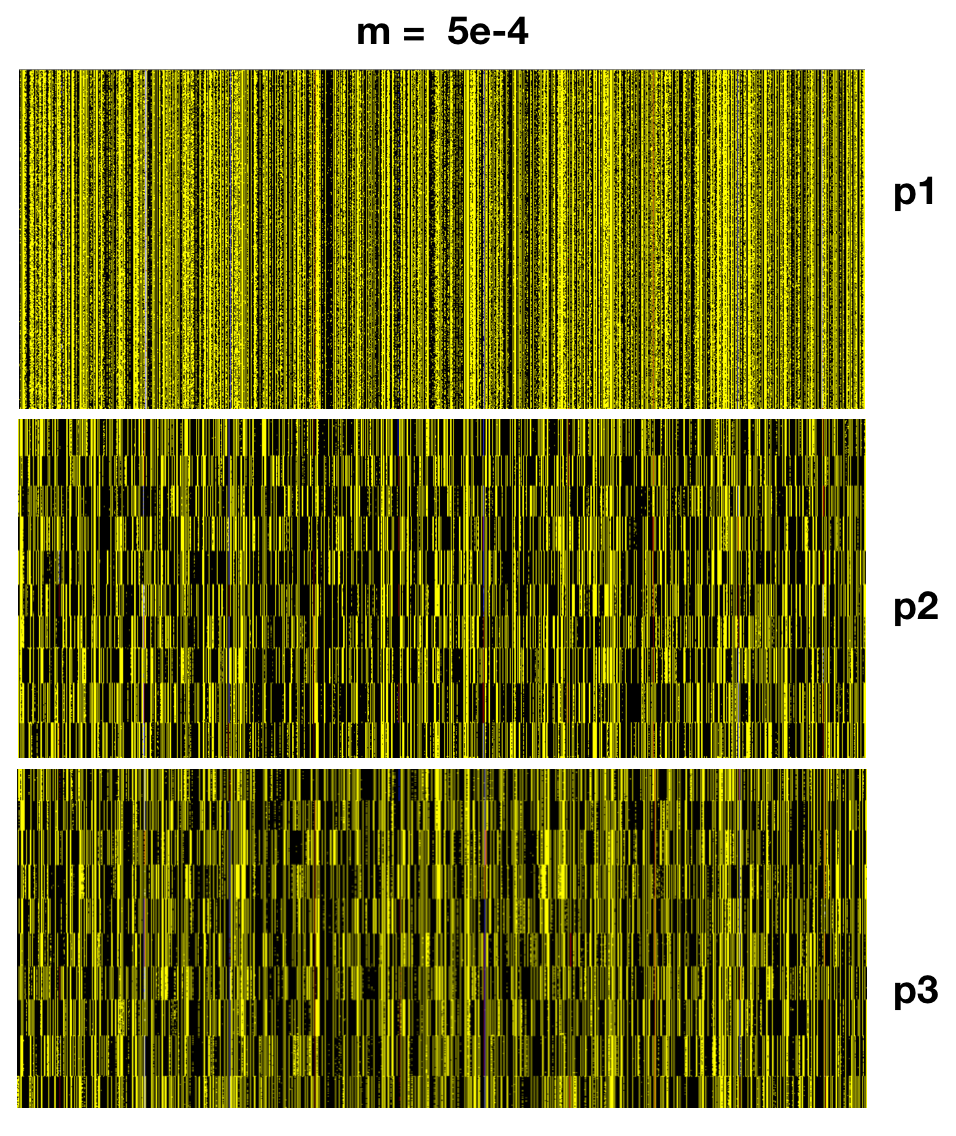
\includegraphics[width=0.7\linewidth]{plotlyPlots/Haplo5e-4.png}
  		\caption{(PLACEHOLDER)
		}
  		\label{fig:Haplo2}
	\end{center}
\end{figure}

\begin{figure}[h!tb]
	\begin{center}
  		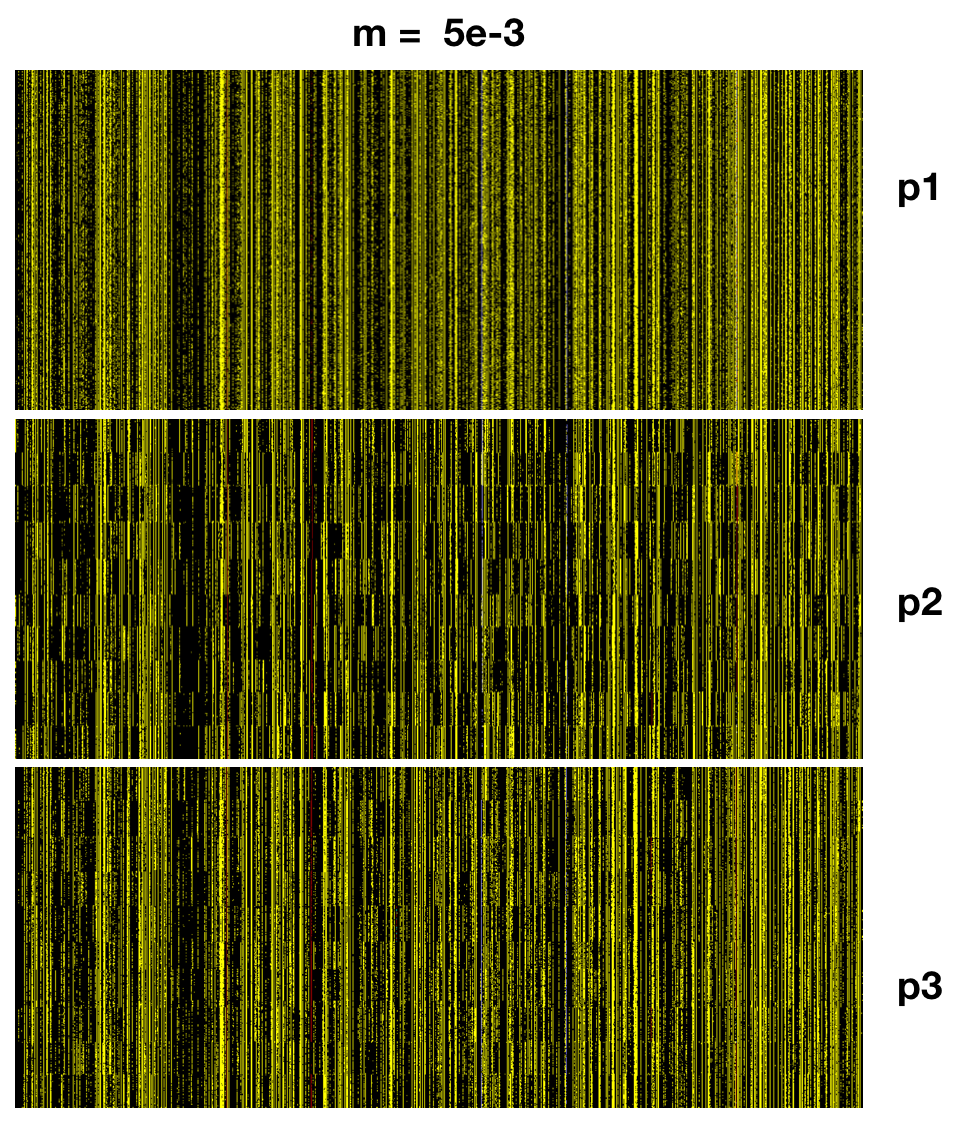
\includegraphics[width=0.7\linewidth]{plotlyPlots/Haplo5e-3.png}
  		\caption{(PLACEHOLDER)
		}
  		\label{fig:Haplo3}
	\end{center}
\end{figure}

\begin{figure}[h!tb]
	\begin{center}
  		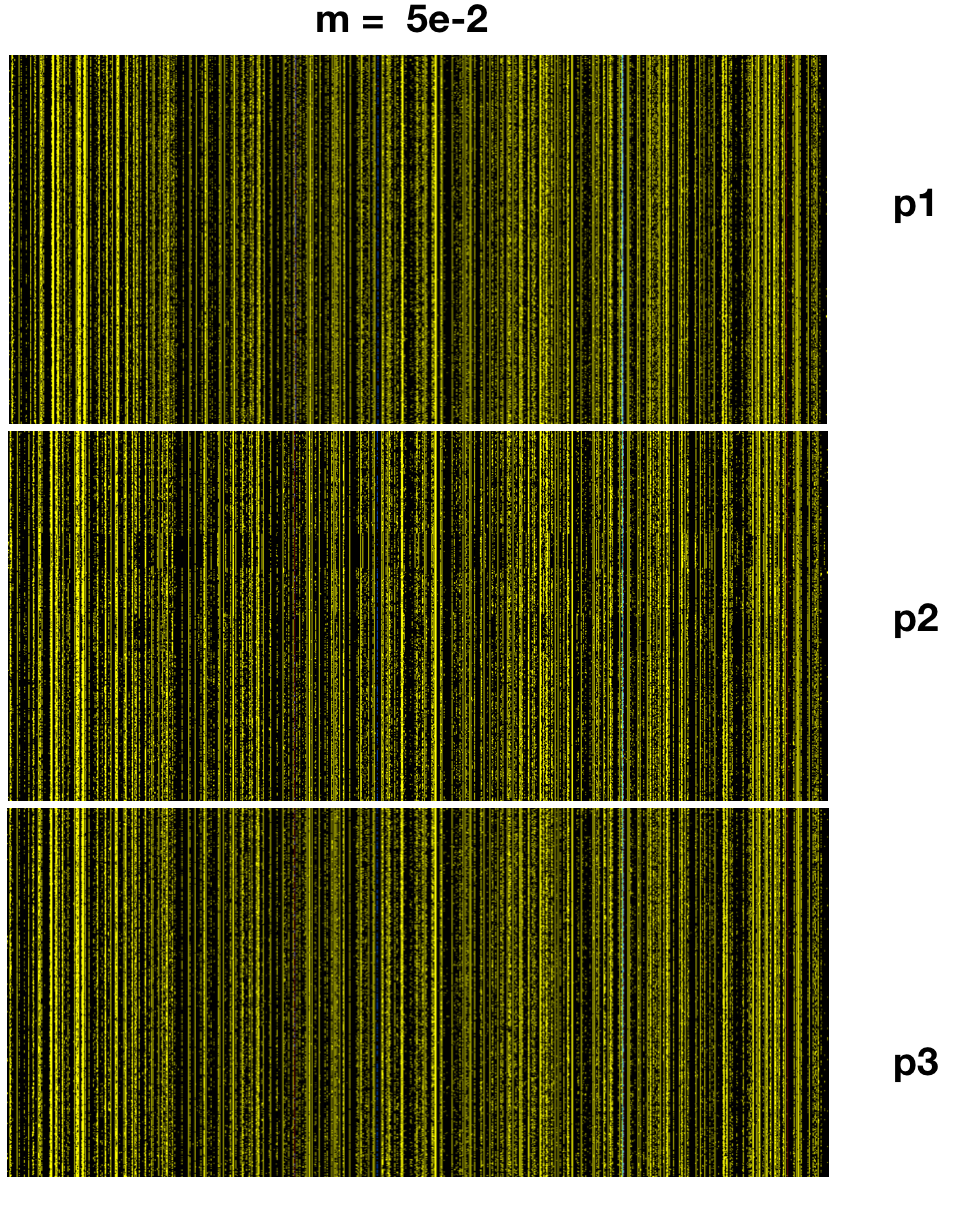
\includegraphics[width=0.7\linewidth]{plotlyPlots/Haplo5e-2.png}
  		\caption{(PLACEHOLDER)
		}
  		\label{fig:Haplo4}
	\end{center}
\end{figure}

\begin{figure}[h!tb]
	\begin{center}
  		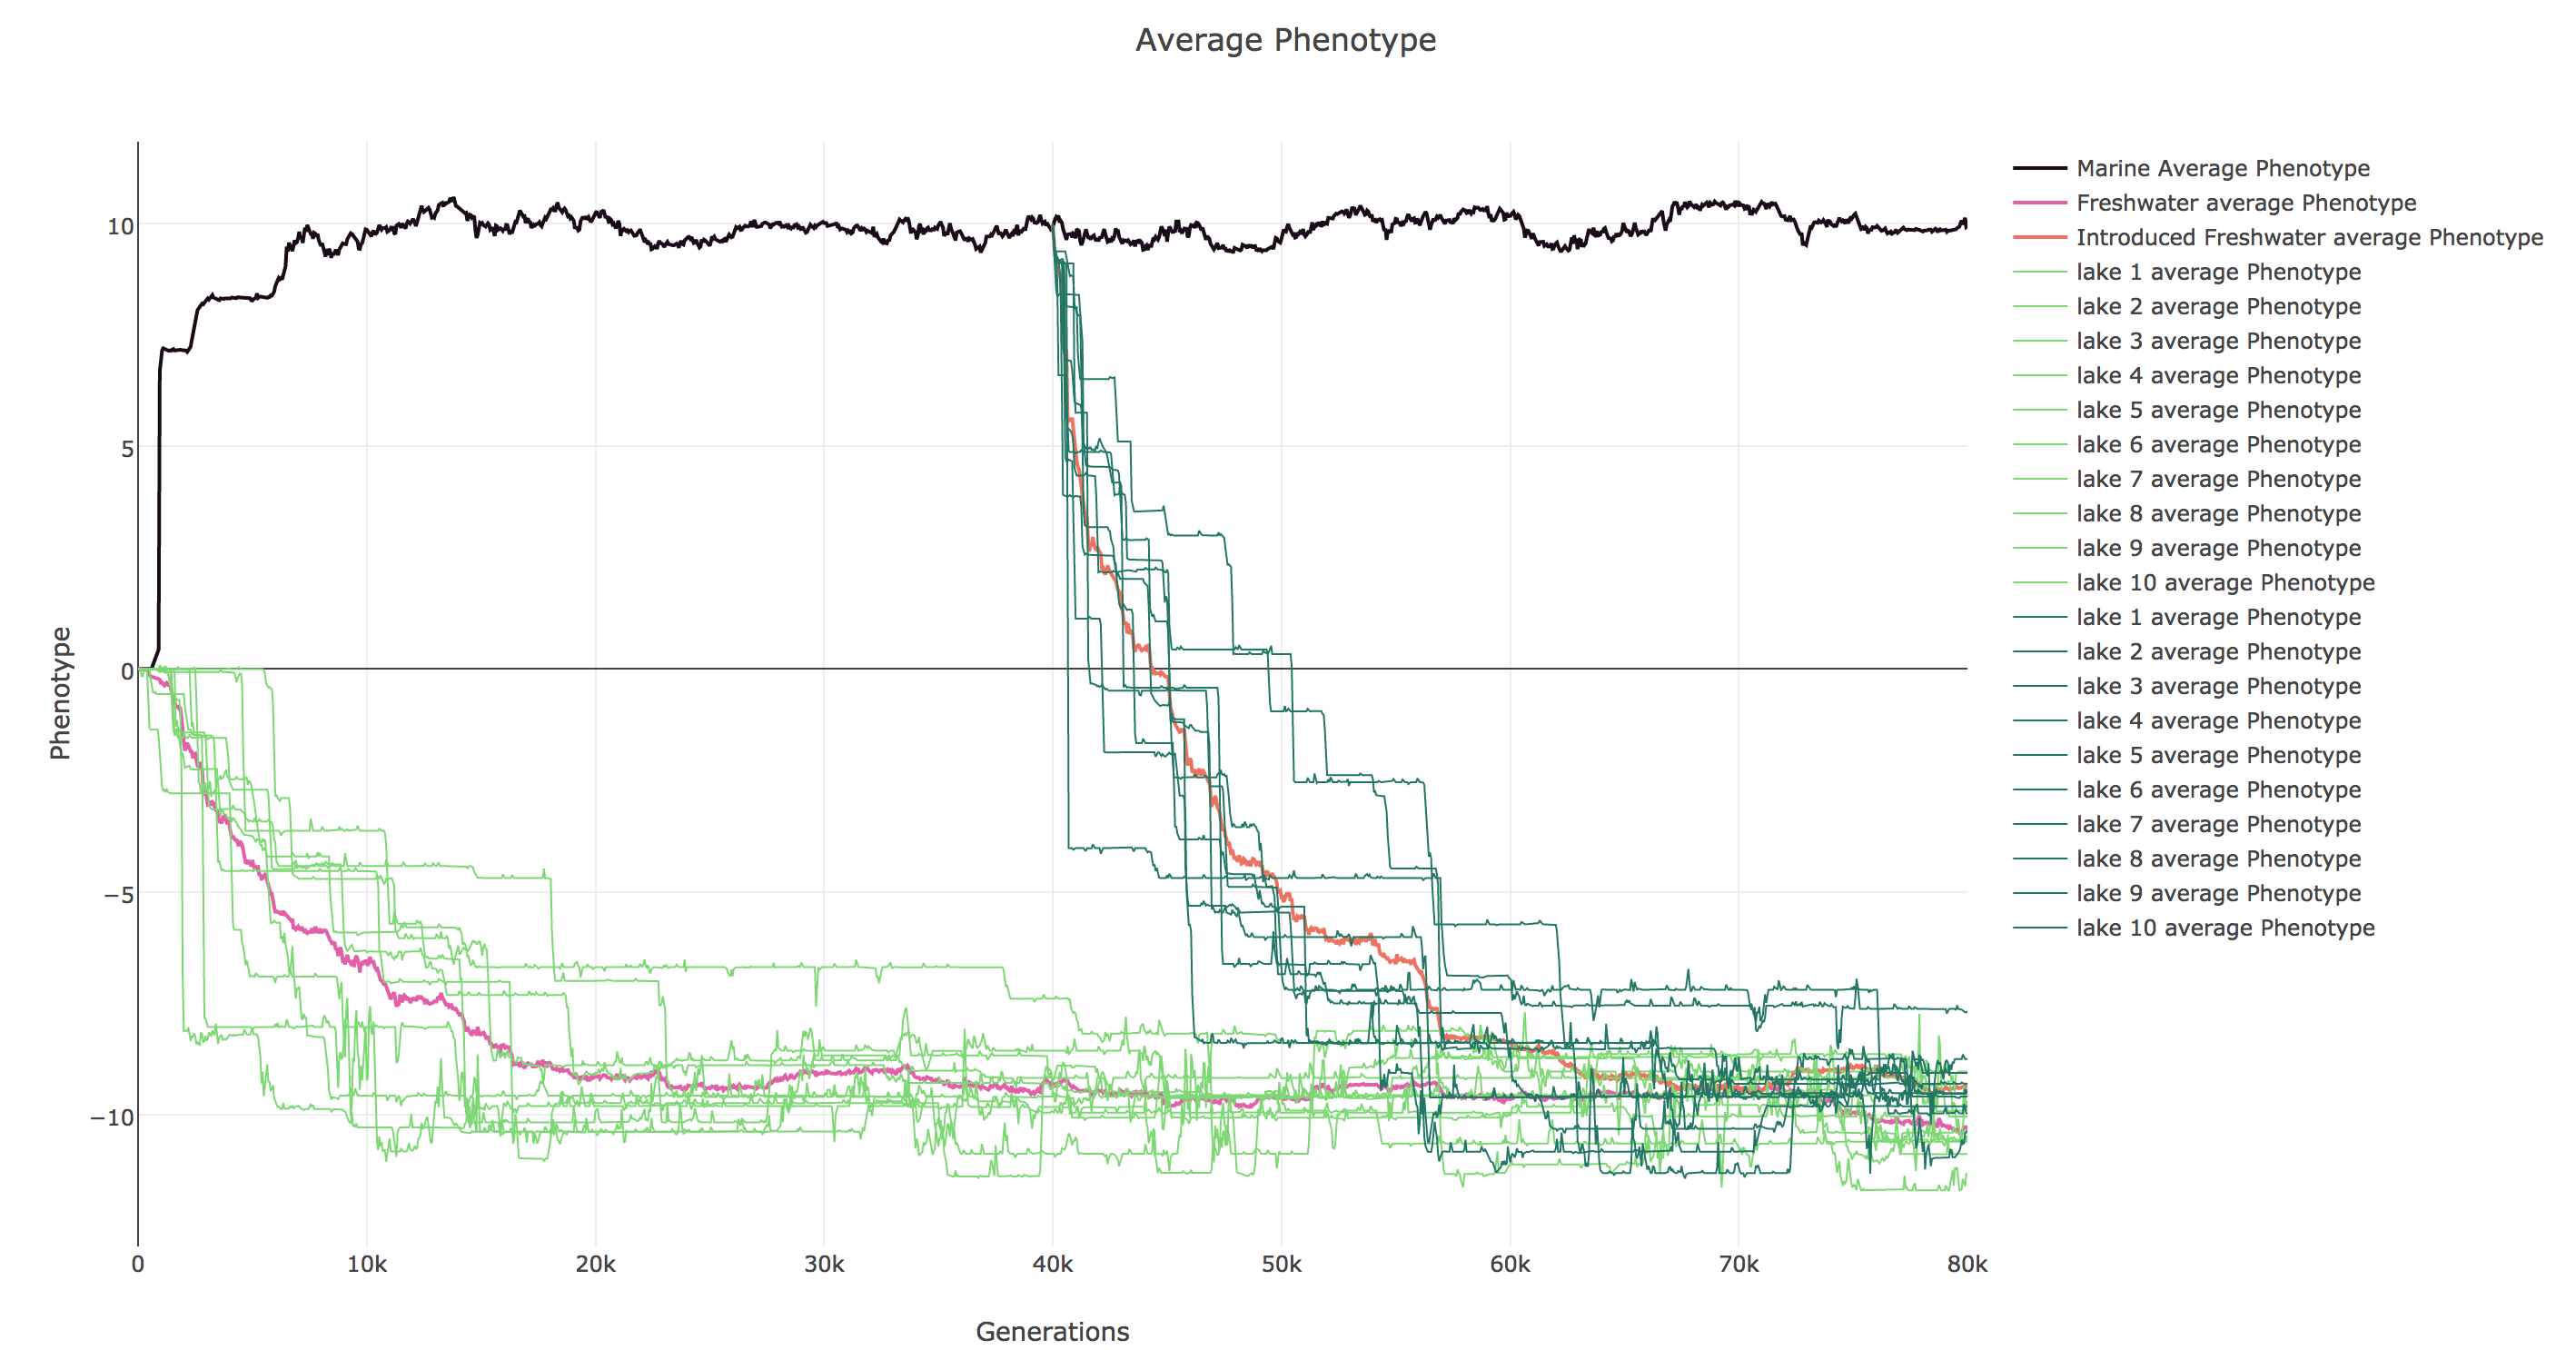
\includegraphics[width=0.7\linewidth]{plotlyPlots/PhenotypeThroughout5e-5.png}
  		\caption{ (PLACEHOLDER)
		}
  		\label{fig:phenotype_ts1}
	\end{center}
\end{figure}

\begin{figure}[h!tb]
	\begin{center}
  		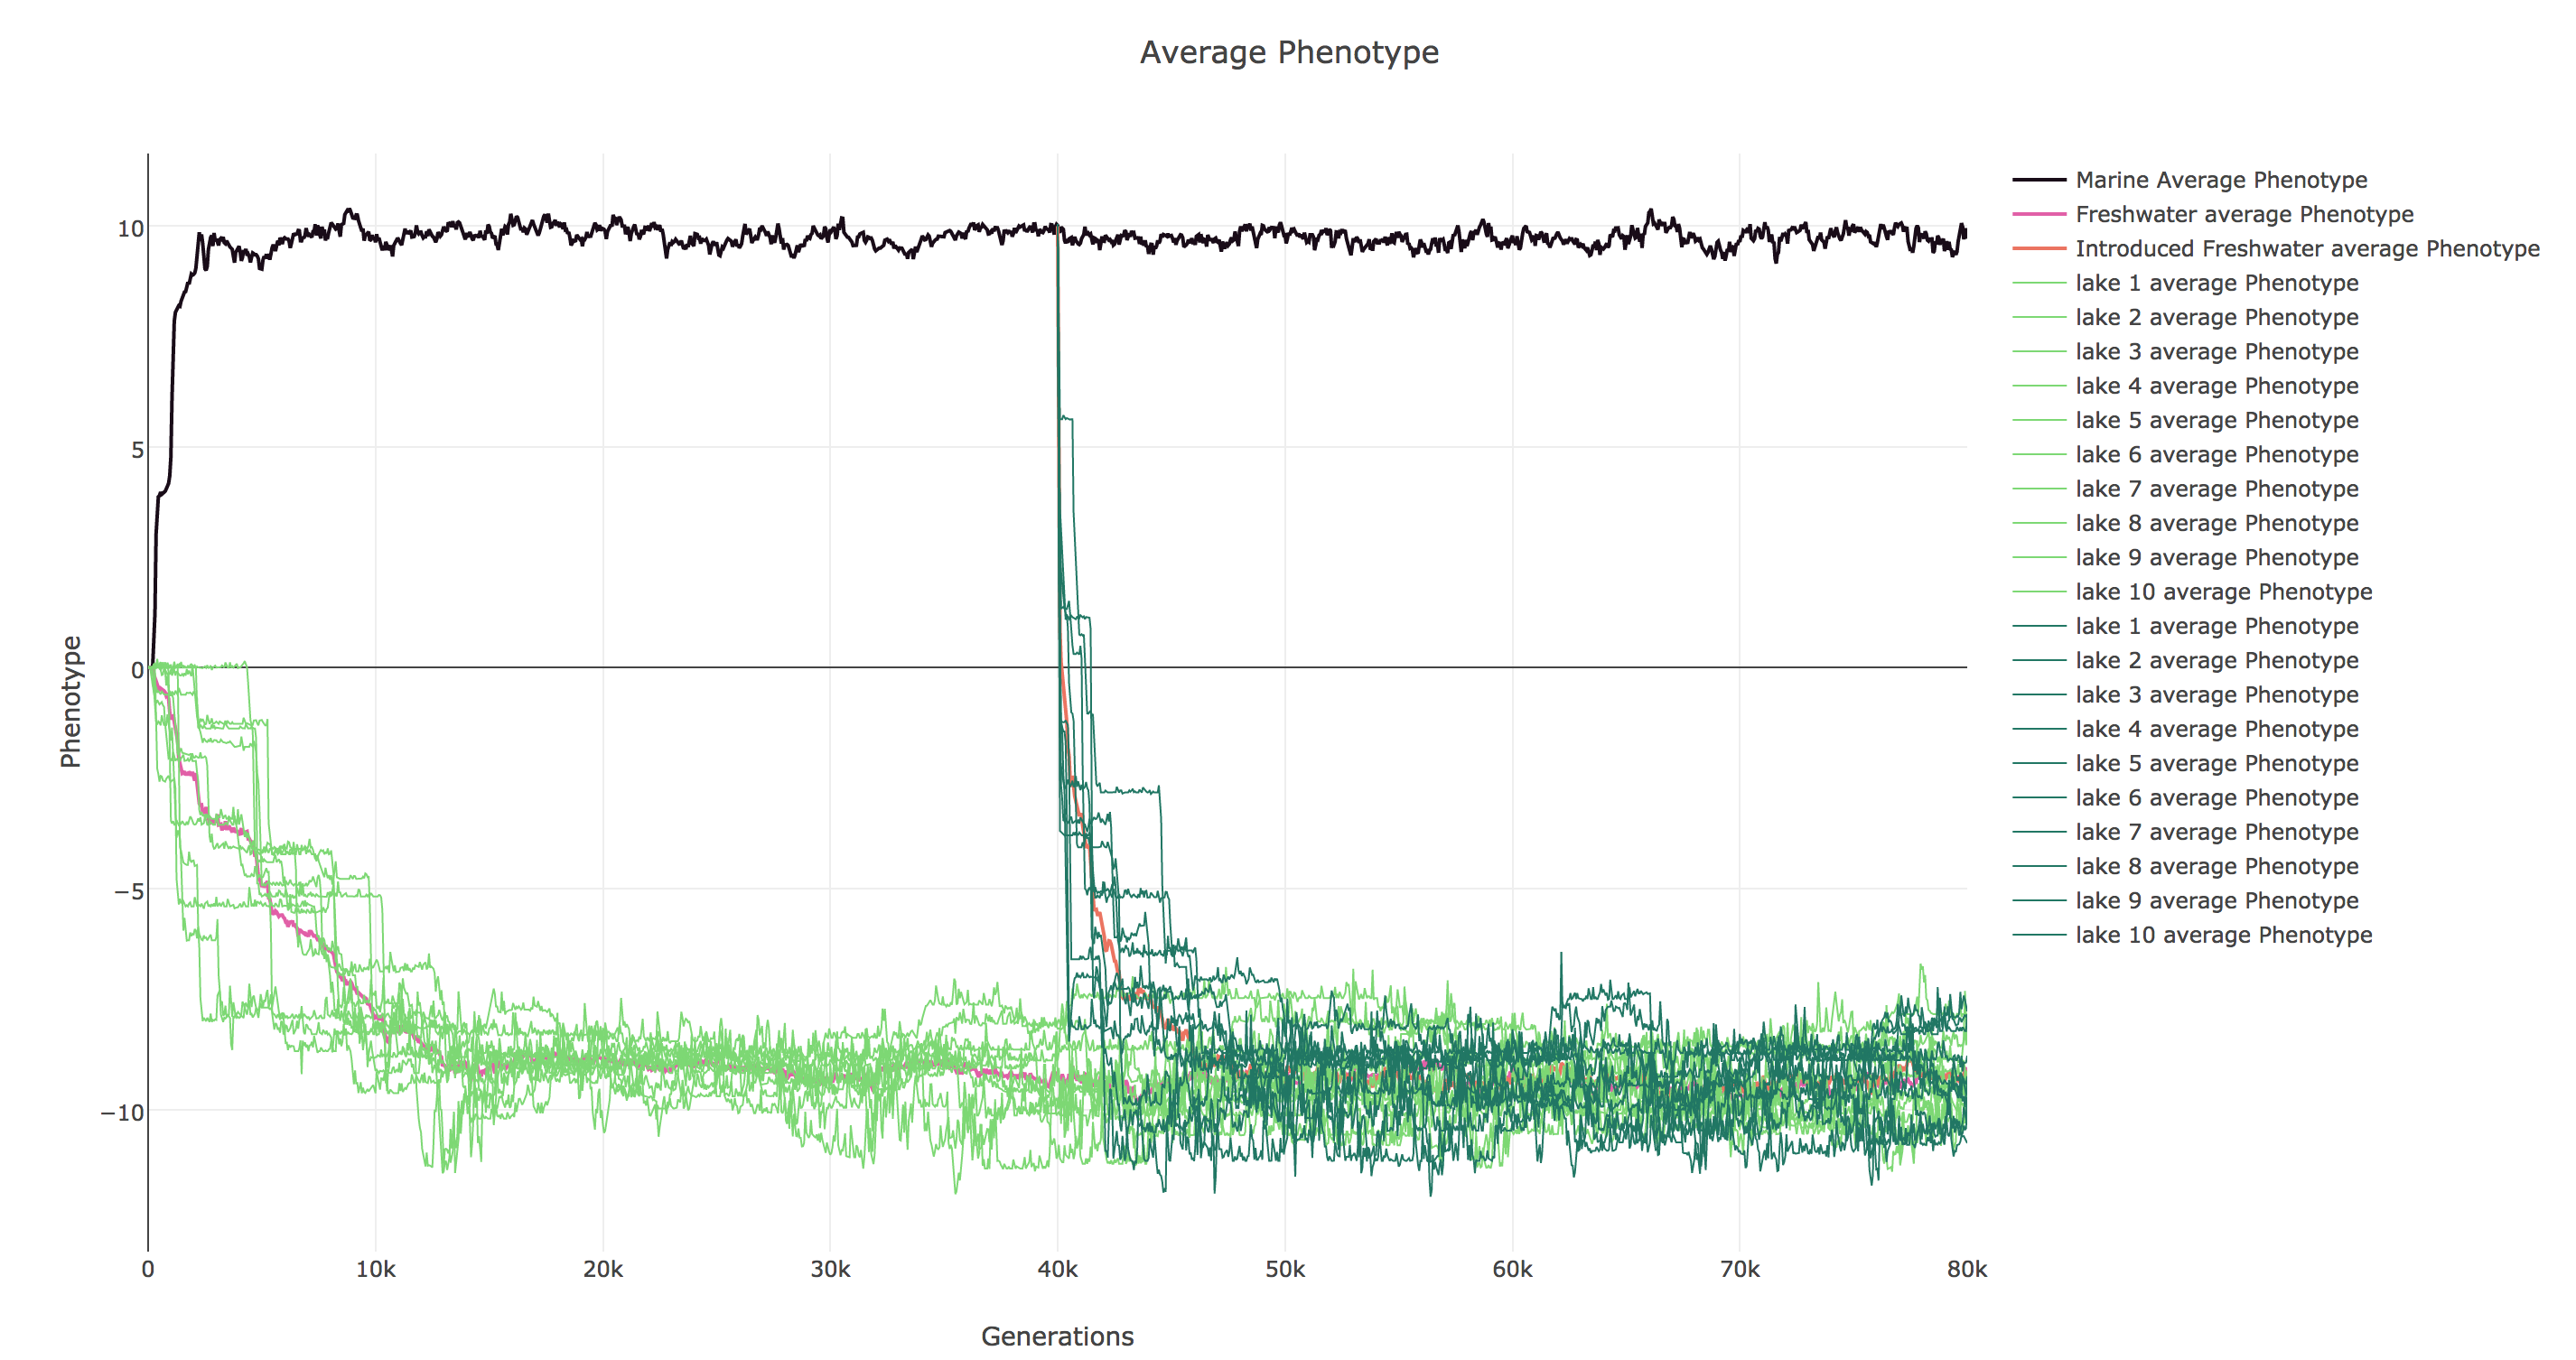
\includegraphics[width=0.7\linewidth]{plotlyPlots/PhenotypeThroughout5e-4.png}
  		\caption{(PLACEHOLDER)
		}
  		\label{fig:phenotype_ts2}
	\end{center}
\end{figure}

\begin{figure}[h!tb]
	\begin{center}
  		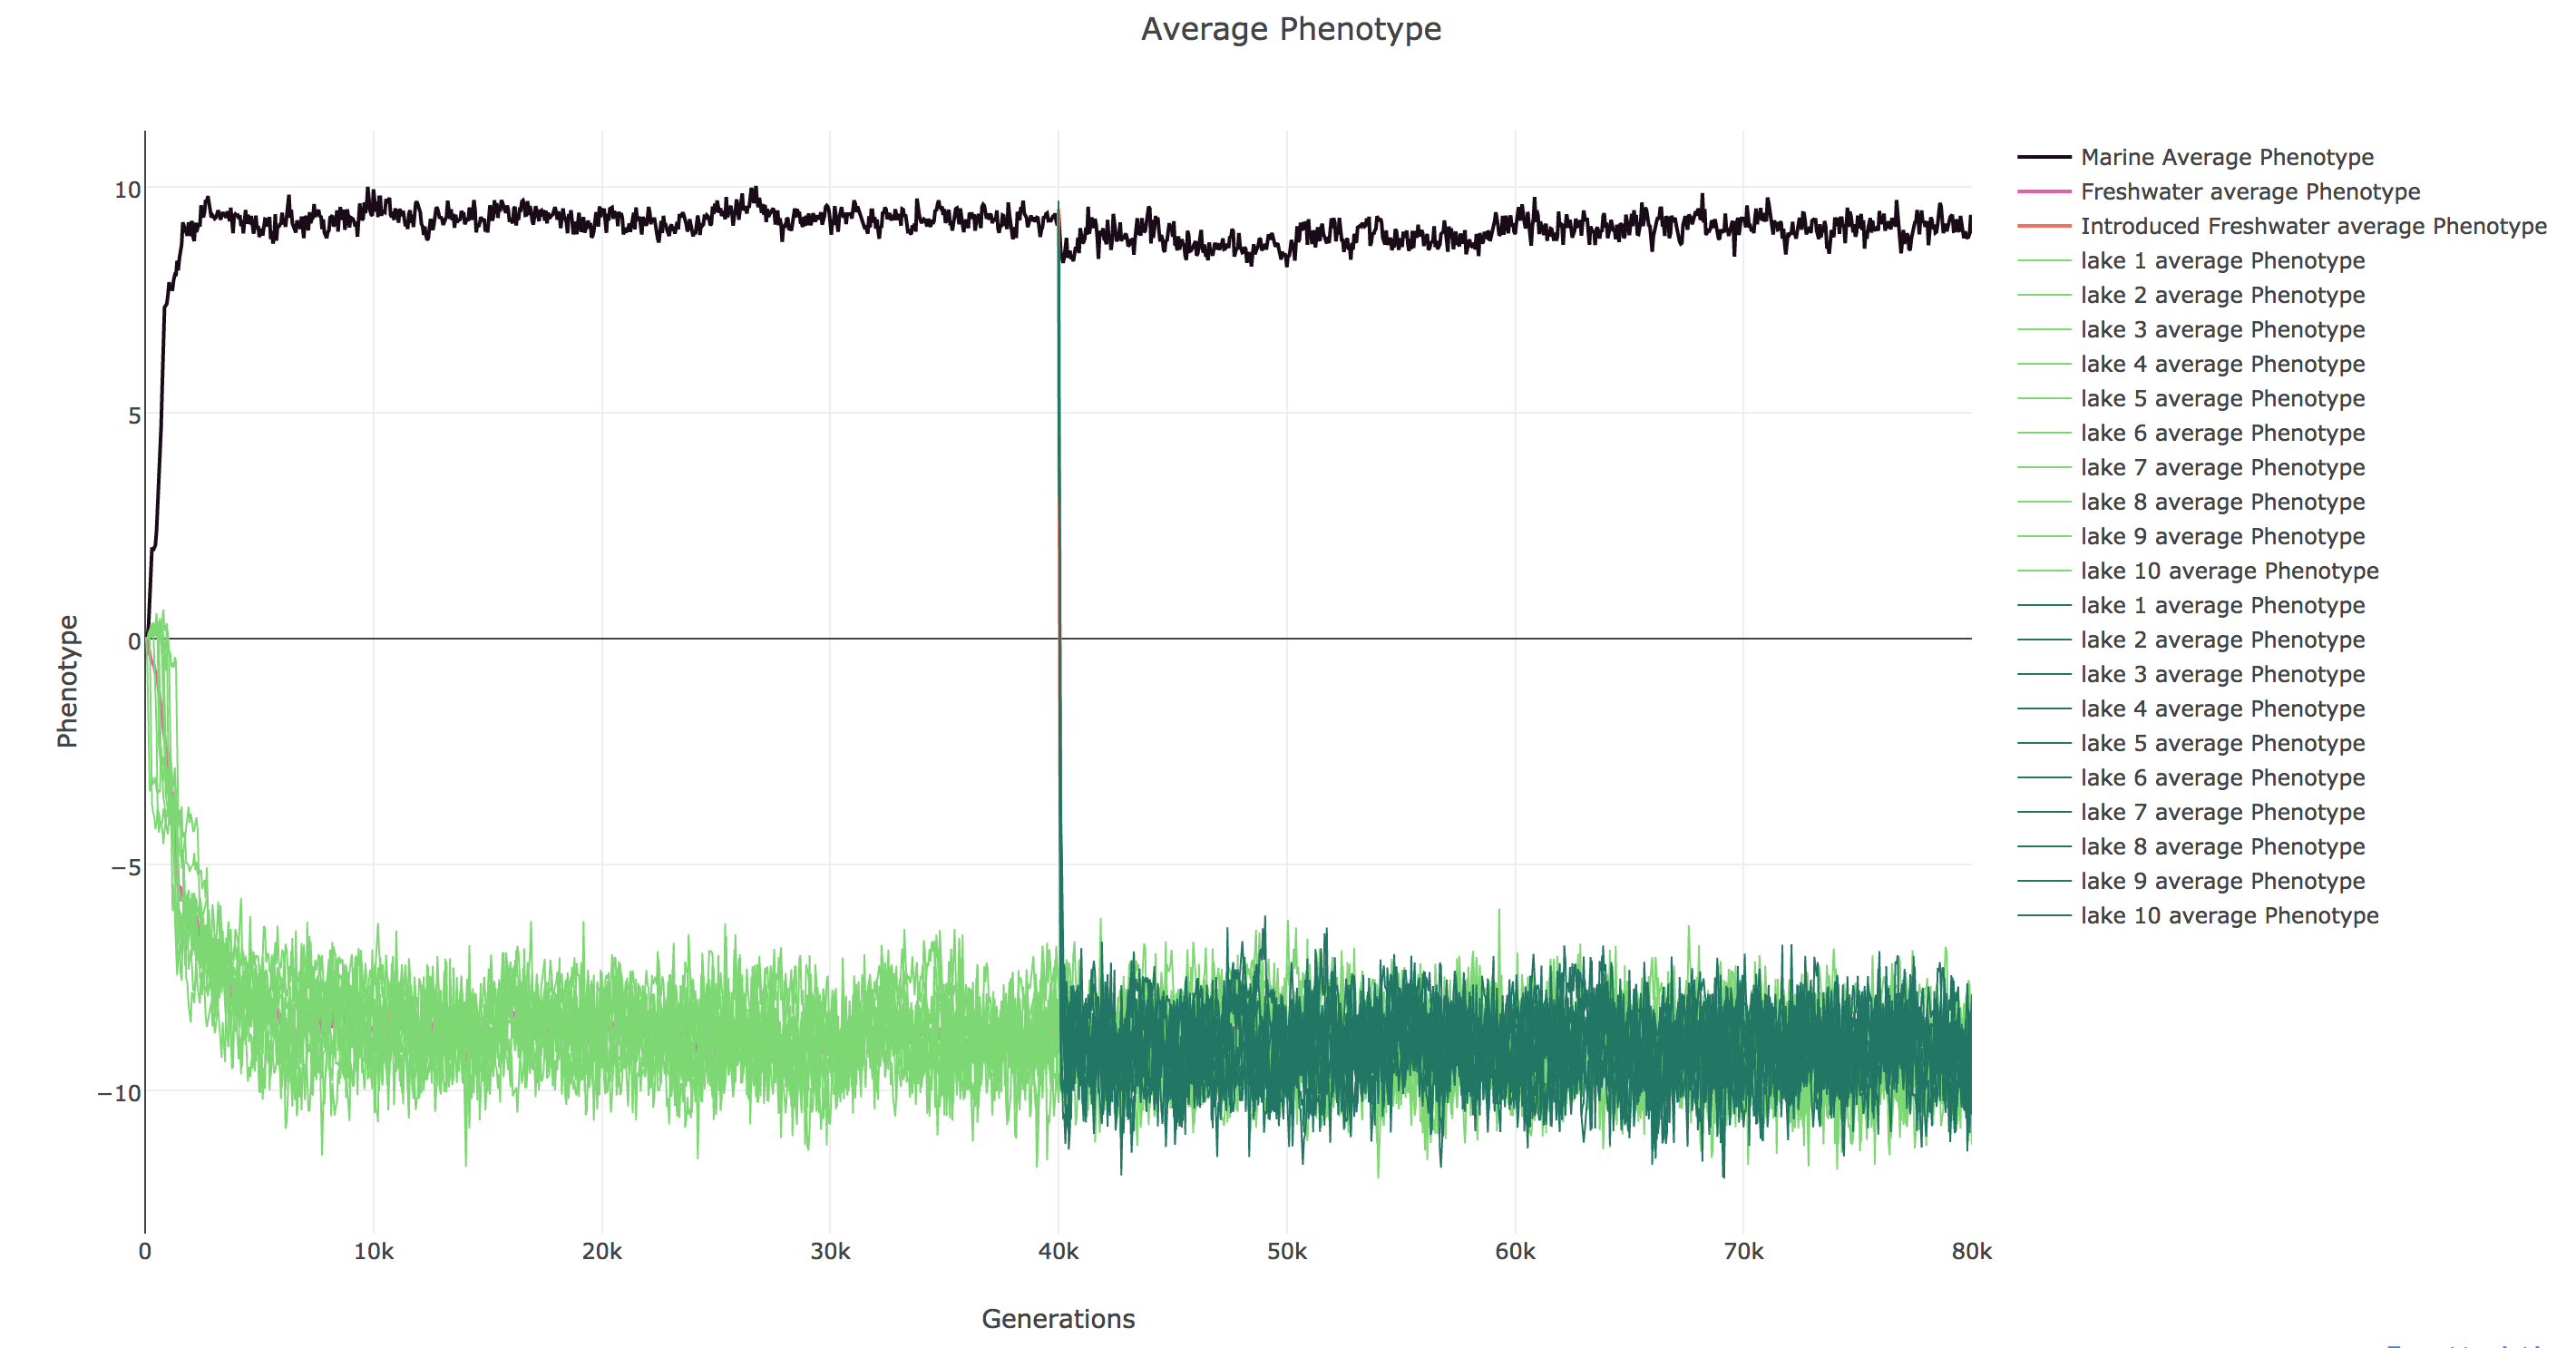
\includegraphics[width=0.7\linewidth]{plotlyPlots/PhenotypeThroughout5e-3.png}
  		\caption{(PLACEHOLDER)
		}
  		\label{fig:phenotype_ts3}
	\end{center}
\end{figure}

\begin{figure}[h!tb]
	\begin{center}
  		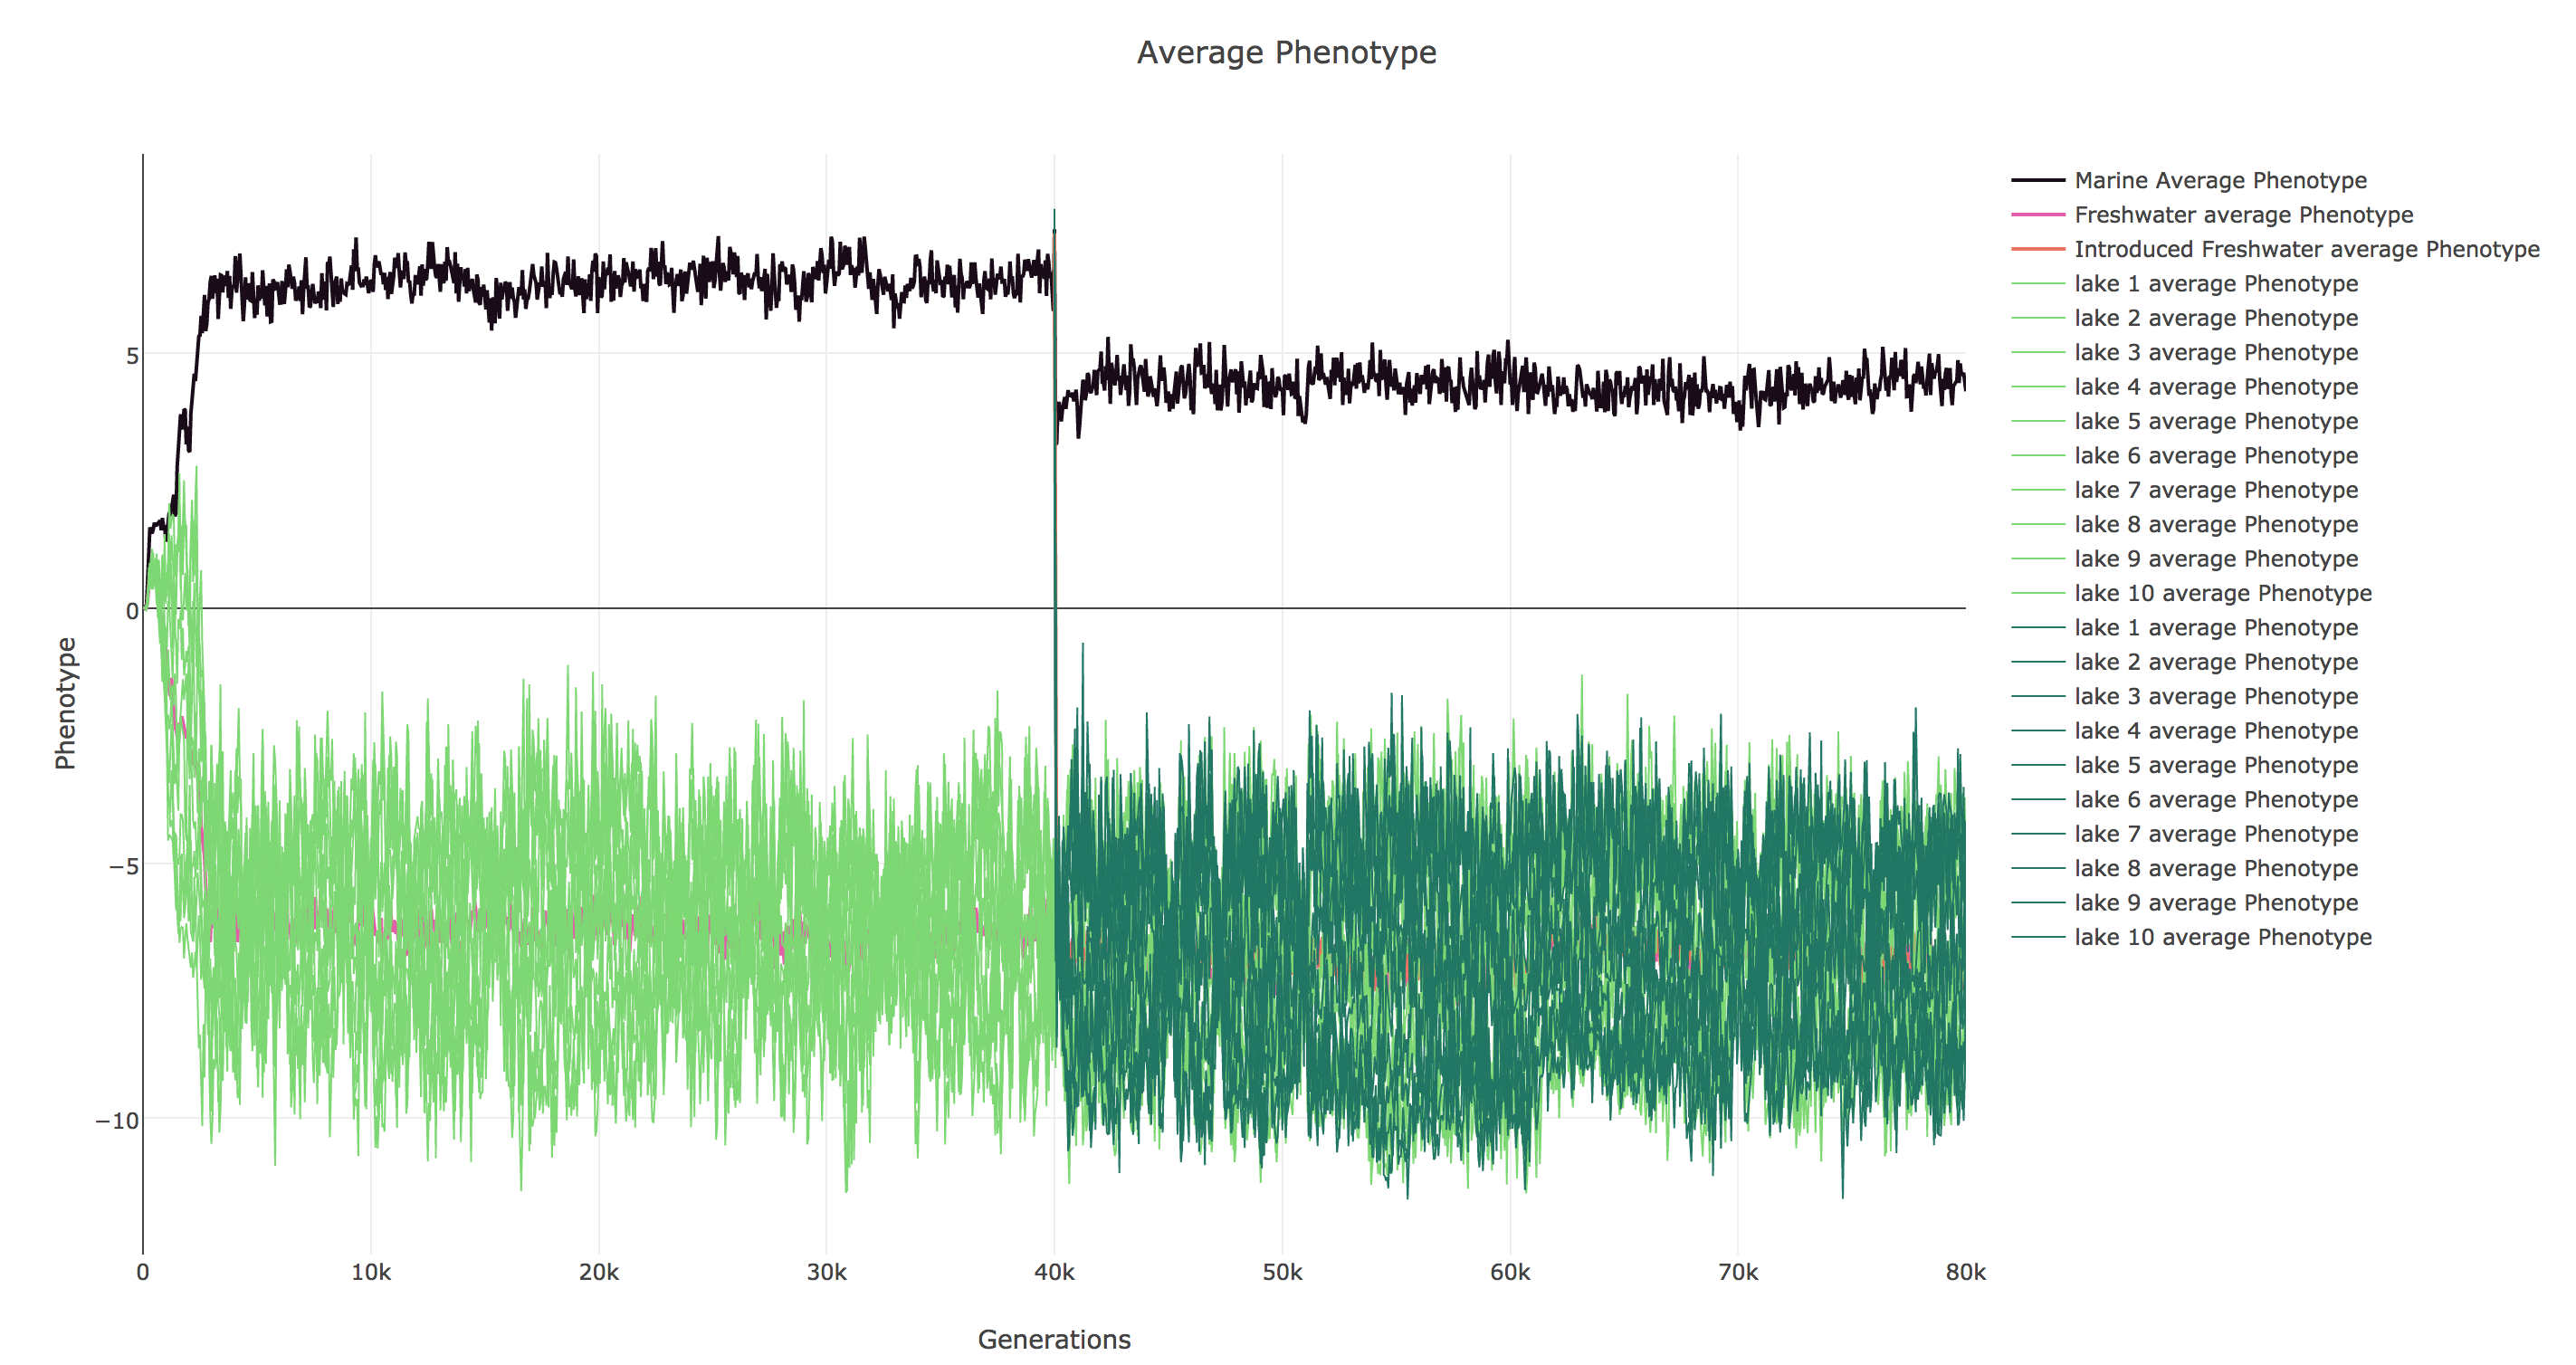
\includegraphics[width=0.7\linewidth]{plotlyPlots/PhenotypeThroughout5e-2.png}
  		\caption{(PLACEHOLDER)
		}
  		\label{fig:phenotype_ts4}
	\end{center}
\end{figure}
\end{comment}

\section{Conclusion \& Discussion}

% at low M we should be able to predict something ---
% at high M we should be able to predict something ----

Here, we suggest a range of migration rate (introgression) parameter values which would allow for the rapid (and in turn, parallel) adaptation 
of marine stickleback introduced intro a freshwater environment.
While this range is heavily effected by all other selections of parameter values. 


\newpage
\plr{some problems because you had bibliographystyle before bibliography}
\bibliographystyle{plainnat}
\bibliography{Citations}{}



\end{document}
